\documentclass[11pt, floatsintext]{article}
\usepackage[vmargin=0.75in, 0.75in]{geometry}
\usepackage{lipsum}
\usepackage[american]{babel}
\usepackage{csquotes}
\usepackage[style=apa,sortcites=true,sorting=nyt,backend=biber]{biblatex}
\DeclareLanguageMapping{american}{american-apa}
\usepackage[colorinlistoftodos]{todonotes}
\usepackage{paralist}
\usepackage{setspace}
\usepackage{longtable}
\usepackage{booktabs}
\usepackage{microtype}
\usepackage{multirow}
\usepackage{adjustbox}
\usepackage{array}
\usepackage{xcolor,colortbl}
\usepackage{threeparttable}
\usepackage{pdflscape}
\usepackage{rotating}
\usepackage{caption}
\captionsetup[table]{
  labelsep=newline,
  justification=justified,
  singlelinecheck=false,
  textfont=it,
}
\captionsetup[figure]{
  justification=justified,
  singlelinecheck=false,
  textfont=up,
}
\definecolor{lavender}{rgb}{0.788, 0.627, 0.863}
\definecolor{lightgreen}{rgb}{0.698, 0.8745, 0.5412}
\definecolor{lightergreen}{cmyk}{.20, 0, .38, 0} %0.13
\newcolumntype{R}[2]{%
    >{\adjustbox{angle=#1,lap=\width-(#2)}\bgroup}%
    l%
    <{\egroup}%
}
\newcommand*\rot{\multicolumn{1}{R{30}{1em}}}
\renewcommand{\thetable}{S\arabic{table}}
\renewcommand{\thefigure}{S\arabic{figure}}
\addbibresource{bibliography.bib}
\usepackage{fancyhdr}
\pagenumbering{roman}
%\fancyhead{SI: Sociolinguistic development in a diverse, multilinguistic environment}
\begin{document}
\thispagestyle{empty}
%\newgeometry{vmargin=1.25in, 1.25in}

\begin{center}
{\hfill}\\
\vspace{20pt}
    \textbf{\large Supplemental Information for:\\ \textit{Sociolinguistic development in a diverse, multilinguistic environment: Evidence from multilingual children in Gujarat, India}}
\end{center}
\vspace{20pt}

%plotted using ggplot
\section*{Participants}
%Our study involved children who tended to be older (7.7--13 years). Given: 
%\begin{inparaenum}[(a)]
    %\item{our participants' more advanced cognitive and linguistic skills,}
    %\item{their enhanced familiarity with thinking about languages, and}
    %\item{our task structure, which enabled children without a strong opinion to opt out of responding, rather than add noise to the data---we hypothesized that we would see even clearer distinctions between languages and better overall understanding in our sample. }
%\end{inparaenum}
\input{tables/child-languages}
\pagebreak
\subsection*{Sample Size Justification}
To determine our sample sizes and anticipate potential effects, we referenced findings from Wagner et al. (\citeyear{wagner2014children}), which examined 4--8-year-old children's ability to categorize different English dialects and to associate them with local vs. non-local cultural artifacts, and from 
Weatherhead et al. (\cite{weatherhead2018accent}), which focused on 4--6-year-old children's geographic inferences based on a speaker's accent, language, and race. 
These studies are similar to (the \textit{Speaker Associations} block of) the current study in that children selected from a constrained set of categorical responses to reflect their inferences about speakers who they heard producing different linguistic variants. 
%Also like our study, each child responded to multiple stimuli from each language variant. 
They differ from ours in that there were always only two responses to obligatorily choose between---one of which was correct, and without the opportunity to opt out---and in that conditions were between-subjects; that is, individual children only responded to a single question for each variant (e.g., ``Was this person born in Canada or born far away?'' for all languages or dialects), or only heard stimuli from a single dialectal contrast (e.g., a child would hear only British and Indian accents, or else only British and American accents, but never all three). 

These studies showed significant differences in children's rates of selecting one option over another in response to different language variants by age 6, in designs with 24--48 children per age group, and 12--24 children per condition. 
They also showed relative consistency \textit{within} children in terms of their responses across multiple trials for the same variant, by roughly the same age. Effect sizes for the effect of dialect on children's associations with cultural items were $\eta^{2}=0.37-0.41$ in Wagner et al. (\citeyear{wagner2014children}), and odds ratios for the effect of language on children's binary responses were between 3.06 and 9.10. 
Thus, we expected medium effect sizes for the effect of language on children's categorical responses. 

We extrapolated target sample sizes informed by these prior results along with %from these prior results, keeping in mind 
three factors that we hypothesized would make effects in our study even more robust. 
First, children in our study tended to be older (7.7--13 years) than previous samples, suggesting more advanced cognitive and linguistic skills. 
Second, children in our study spoke, studied, and heard multiple languages in their day-to-day lives, which might mean enhanced familiarity with thinking about languages. 
Third, children in our study could opt out of responding when they did not have a strong opinion for a given question, rather than add noise to the data. 
In light of these factors, we aimed for at least 24 children per age group. 
For the older two age groups (5th- and 7th-graders), we were able to collect data from sample sizes at the higher end of the range established by previous studies (\textit{n}s=48 and 55, respectively). 
Running the study with the 3rd-graders took significantly longer, resulting in a smaller sample size for that age group ($n=27$). 
%\pagebreak
%\section*{Speaker Association Means}
% MEANS
\begin{table}[t]
%\vspace{-50pt}
 \centering
\caption{Mean Geographic Origin Association by Speaker Language and Child Grade}
\begin{footnotesize}
\renewcommand{\tabcolsep}{0.15cm}
\label{tab:geographic-origins-means}
\begin{tabular}{p{.1in}lrrrrrrrrr}
\toprule
 &  & \multicolumn{3}{c}{3rd} & \multicolumn{3}{c}{5th} & \multicolumn{3}{c}{7th} \\
\cline{3-5} \cline{6-8} \cline{9-11}
&  & \textit{n} & \textit{M} & [95\% \textit{CI}] &  \textit{n} & \textit{M} & [95\% \textit{CI}] &  \textit{n}  & \textit{M} & [95\% \textit{CI}]\\
\midrule
\multicolumn{11}{l}{\textbf{Gujarat (Same State as Me)}}\\
 & Gujarati & 17 & 0.44 & [0.28, 0.6] & 72 & 0.74 & [0.65, 0.82] & 72 & 0.77 & [0.69, 0.85]\\

 & Hindi & 31 & 0.79 & [0.66, 0.92] & 48 & 0.49 & [0.4, 0.59] & 63 & 0.68 & [0.59, 0.77]\\

 & Urdu & 26 & 0.68 & [0.53, 0.84] & 49 & 0.51 & [0.4, 0.61] & 55 & 0.59 & [0.48, 0.68]\\

 & Marathi & 16 & 0.41 & [0.26, 0.56] & 28 & 0.29 & [0.2, 0.38] & 31 & 0.33 & [0.25, 0.43]\\

 & Tamil & 12 & 0.31 & [0.17, 0.45] & 15 & 0.15 & [0.08, 0.24] & 6 & 0.06 & [0.02, 0.12]\\

 & English (India) & 12 & 0.32 & [0.17, 0.47] & 10 & 0.10 & [0.04, 0.17] & 10 & 0.11 & [0.05, 0.17]\\

 & English (U.S.) & 11 & 0.28 & [0.15, 0.43] & 5 & 0.05 & [0.01, 0.1] & 8 & 0.08 & [0.03, 0.15]\\

& Mandarin & 4 & 0.10 & [0.02, 0.21] & 4 & 0.04 & [0.01, 0.08] & 1 & 0.01 & [0, 0.03]\\

\midrule
\multicolumn{11}{l}{\textbf{India (Different State)}}\\
  & Gujarati & 8 & 0.21 & [0.08, 0.35] & 16 & 0.16 & [0.1, 0.24] & 14 & 0.15 & [0.09, 0.23]\\

 & Hindi & 3 & 0.08 & [0, 0.17] & 46 & 0.47 & [0.38, 0.57] & 29 & 0.31 & [0.22, 0.41]\\

 & Urdu & 8 & 0.21 & [0.1, 0.34] & 42 & 0.43 & [0.33, 0.54] & 33 & 0.35 & [0.26, 0.46]\\

 & Marathi & 13 & 0.33 & [0.19, 0.49] & 54 & 0.56 & [0.46, 0.65] & 56 & 0.60 & [0.5, 0.71]\\

 & Tamil & 17 & 0.44 & [0.29, 0.59] & 51 & 0.53 & [0.43, 0.63] & 67 & 0.71 & [0.62, 0.8]\\

 & English (India) & 6 & 0.16 & [0.05, 0.28] & 18 & 0.19 & [0.11, 0.27] & 19 & 0.20 & [0.13, 0.29]\\

 & English (U.S.) & 11 & 0.28 & [0.14, 0.43] & 25 & 0.26 & [0.18, 0.35] & 14 & 0.15 & [0.08, 0.22]\\

& Mandarin & 7 & 0.18 & [0.07, 0.32] & 19 & 0.20 & [0.12, 0.28] & 19 & 0.20 & [0.13, 0.28]\\

\midrule
\multicolumn{11}{l}{\textbf{Foreign (Outside India)}}\\
& Gujarati & 13 & 0.33 & [0.19, 0.49] & 9 & 0.09 & [0.04, 0.15] & 7 & 0.08 & [0.02, 0.13]\\

 & Hindi & 5 & 0.13 & [0.03, 0.24] & 2 & 0.02 & [0, 0.05] & 0 & --- & ---\\

 & Urdu & 3 & 0.08 & [0, 0.18] & 4 & 0.04 & [0.01, 0.08] & 4 & 0.04 & [0.01, 0.09]\\

 & Marathi & 9 & 0.23 & [0.1, 0.38] & 14 & 0.14 & [0.08, 0.22] & 4 & 0.04 & [0.01, 0.09]\\

 & Tamil & 10 & 0.26 & [0.12, 0.38] & 30 & 0.31 & [0.21, 0.4] & 14 & 0.15 & [0.09, 0.22]\\

 & English (India) & 18 & 0.47 & [0.32, 0.63] & 68 & 0.71 & [0.61, 0.8] & 63 & 0.67 & [0.59, 0.77]\\

 & English (U.S.) & 16 & 0.41 & [0.27, 0.56] & 65 & 0.67 & [0.58, 0.77] & 70 & 0.74 & [0.64, 0.82]\\

& Mandarin & 25 & 0.64 & [0.47, 0.79] & 71 & 0.73 & [0.64, 0.82] & 70 & 0.75 & [0.67, 0.83]\\

\midrule
\multicolumn{11}{l}{\textbf{No Opinion}}\\
& Gujarati & 1 & 0.03 & [0, 0.08] & 0 & --- & --- & 0 & --- & ---\\

 & Hindi & 0 & --- & --- & 1 & 0.01 & [0, 0.03] & 1 & 0.01 & [0, 0.03]\\

 & Urdu & 1 & 0.03 & [0, 0.09] & 2 & 0.02 & [0, 0.05] & 2 & 0.02 & [0, 0.05]\\

 & Marathi & 1 & 0.03 & [0, 0.08] & 1 & 0.01 & [0, 0.03] & 2 & 0.02 & [0, 0.05]\\

 & Tamil & 0 & --- & --- & 1 & 0.01 & [0, 0.03] & 7 & 0.07 & [0.03, 0.13]\\

 & English (India) & 2 & 0.05 & [0, 0.14] & 0 & --- & --- & 2 & 0.02 & [0, 0.05]\\

 & English (U.S.) & 1 & 0.03 & [0, 0.08] & 2 & 0.02 & [0, 0.05] & 3 & 0.03 & [0, 0.07]\\

& Mandarin & 3 & 0.08 & [0, 0.17] & 3 & 0.03 & [0, 0.07] & 3 & 0.03 & [0, 0.08]\\
\bottomrule
\end{tabular}
\end{footnotesize}
\end{table}

\thispagestyle{empty}
\begin{table}[H]
\vspace{-20pt}
\centering
\caption{Mean Religious Association by Speaker Language and Child Grade}\label{tab:religion-means}\\
\begin{footnotesize}
%\renewcommand{\tabcolsep}{0.15cm}
\begin{tabular}{p{.1in}lrrrrrrrrr}
%\begin{tabular}{p{.1in}lrrrrrrrrr}
\toprule
 &  & \multicolumn{3}{c}{\textbf{3rd}} & \multicolumn{3}{c}{\textbf{5th}} & \multicolumn{3}{c}{\textbf{7th}} \\
\cline{3-5} \cline{6-8} \cline{9-11}\\[-.75em]
&  & \textit{n} & \textit{M} & [95\% \textit{CI}] &  \textit{n} & \textit{M} & [95\% \textit{CI}] &  \textit{n}  & \textit{M} & [95\% \textit{CI}]\\
\midrule
\multicolumn{11}{l}{\textbf{Hindu}}\\
 & Gujarati & 12 & 0.32 & [0.18, 0.49] & 72 & 0.71 & [0.61, 0.79] & 67 & 0.71 & [0.62, 0.80]\\

 & Hindi & 11 & 0.29 & [0.14, 0.43] & 54 & 0.53 & [0.45, 0.63] & 50 & 0.53 & [0.44, 0.63]\\

 & Urdu & 12 & 0.33 & [0.19, 0.48] & 46 & 0.46 & [0.36, 0.55] & 44 & 0.47 & [0.38, 0.57]\\

 & Marathi & 7 & 0.18 & [0.07, 0.32] & 48 & 0.48 & [0.38, 0.57] & 56 & 0.60 & [0.50, 0.69]\\

 & Tamil & 9 & 0.24 & [0.12, 0.38] & 17 & 0.17 & [0.10, 0.25] & 10 & 0.11 & [0.05, 0.17]\\

 & English (India) & 10 & 0.27 & [0.14, 0.42] & 15 & 0.15 & [0.08, 0.23] & 9 & 0.10 & [0.04, 0.16]\\

 & English (U.S.) & 8 & 0.21 & [0.08, 0.35] & 5 & 0.05 & [0.01, 0.09] & 7 & 0.07 & [0.02, 0.13]\\

& Mandarin & 4 & 0.11 & [0.02, 0.21] & 3 & 0.03 & [0.00, 0.07] & 0 & --- & ---\\

\midrule
\multicolumn{11}{l}{\textbf{Muslim}}\\
 & Gujarati & 10 & 0.27 & [0.14, 0.41] & 7 & 0.07 & [0.03, 0.12] & 11 & 0.12 & [0.05, 0.18]\\

 & Hindi & 19 & 0.50 & [0.33, 0.66] & 34 & 0.34 & [0.25, 0.43] & 26 & 0.28 & [0.19, 0.36]\\

 & Urdu & 21 & 0.58 & [0.42, 0.74] & 40 & 0.40 & 0.30, 0.49] & 39 & 0.42 & [0.32, 0.53]\\

 & Marathi & 9 & 0.24 & [0.11, 0.37] & 10 & 0.10 & [0.05, 0.16] & 1 & 0.01 & [0.00, 0.03]\\

 & Tamil & 9 & 0.24 & [0.10, 0.37] & 11 & 0.11 & [0.05, 0.18] & 6 & 0.06 & [0.02, 0.12]\\

 & English (India) & 5 & 0.14 & [0.03, 0.26] & 12 & 0.12 & [0.06, 0.19] & 1 & 0.01 & [0.00, 0.03]\\

 & English (U.S.) & 4 & 0.11 & [0.03, 0.21] & 13 & 0.13 & [0.07, 0.20] & 3 & 0.03 & [0.00, 0.07]\\
 & Mandarin & 4 & 0.11 & [0.02, 0.21] & 9 & 0.09 & [0.04, 0.15] & 6 & 0.06 & [0.02, 0.12]\\
 \midrule
\multicolumn{11}{l}{\textbf{Jain}}\\
  & Gujarati & 7 & 0.19 & [0.08, 0.32] & 10 & 0.10 & [0.05, 0.16] & 3 & 0.03 & [0.00, 0.06]\\

 & Hindi & 4 & 0.11 & [0.02, 0.21] & 8 & 0.08 & [0.03, 0.14] & 9 & 0.10 & [0.04, 0.15]\\

 & Urdu & 0 & --- & --- & 10 & 0.10 & [0.04, 0.16] & 3 & 0.03 & [0.00, 0.07]\\

 & Marathi & 8 & 0.21 & [0.09, 0.34] & 16 & 0.16 & [0.09, 0.23] & 5 & 0.05 & [0.02, 0.11]\\

 & Tamil & 7 & 0.18 & [0.06, 0.31] & 30 & 0.30 & [0.22, 0.39] & 18 & 0.19 & [0.12, 0.27]\\

 & English (India) & 6 & 0.16 & [0.05, 0.30] & 16 & 0.16 & [0.10, 0.23] & 6 & 0.07 & [0.02, 0.12]\\

 & English (U.S.) & 5 & 0.13 & [0.03, 0.24] & 20 & 0.20 & [0.12, 0.28] & 5 & 0.05 & [0.01, 0.09]\\

& Mandarin & 7 & 0.18 & [0.07, 0.31] & 18 & 0.18 & [0.11, 0.26] & 12 & 0.13 & [0.07, 0.20]\\
 \midrule
\multicolumn{11}{l}{\textbf{Christian}}\\
 & Gujarati & 5 & 0.14 & [0.03, 0.26] & 4 & 0.04 & [0.01, 0.08] & 3 & 0.03 & [0.00, 0.07]\\

 & Hindi & 0 & --- & --- & 4 & 0.04 & [0.01, 0.08] & 1 & 0.01 & [0.00, 0.03]\\

 & Urdu & 4 & 0.11 & [0.02, 0.22] & 3 & 0.03 & [0.00, 0.07] & 0 & --- & ---\\

 & Marathi & 6 & 0.16 & [0.05, 0.28] & 8 & 0.08 & [0.03, 0.14] & 4 & 0.04 & [0.01, 0.09]\\

 & Tamil & 8 & 0.21 & [0.08, 0.35] & 16 & 0.16 & [0.09, 0.24] & 5 & 0.05 & [0.01, 0.11]\\

 & English (India) & 12 & 0.32 & [0.18, 0.48] & 32 & 0.32 & [0.24, 0.41] & 48 & 0.52 & [0.42, 0.62]\\

 & English (U.S.) & 14 & 0.37 & [0.22, 0.52] & 36 & 0.36 & [0.27, 0.46] & 40 & 0.42 & [0.33, 0.52]\\
& Mandarin & 10 & 0.26 & [0.14, 0.41] & 20 & 0.20 & [0.13, 0.28] & 21 & 0.23 & [0.15, 0.31]\\
 \midrule
\multicolumn{11}{l}{\textbf{Buddhist}}\\
& Gujarati & 3 & 0.08 & [0.00, 0.18] & 4 & 0.04 & [0.01, 0.08] & 3 & 0.03 & [0.00, 0.07]\\

 & Hindi & 3 & 0.08 & [0.00, 0.18] & 0 & --- & --- & 2 & 0.02 & [0.00, 0.05]\\

 & Urdu & 0 & --- & --- & 1 & 0.01 & [0.00, 0.03] & 3 & 0.03 & [0.00, 0.07]\\

 & Marathi & 5 & 0.13 & [0.05, 0.25] & 10 & 0.10 & [0.05, 0.16] & 14 & 0.15 & [0.07, 0.22]\\

 & Tamil & 2 & 0.05 & [0.00, 0.13] & 18 & 0.18 & [0.11, 0.25] & 31 & 0.33 & [0.23, 0.43]\\

 & English (India) & 1 & 0.03 & [0.00, 0.09] & 7 & 0.07 & [0.03, 0.13] & 4 & 0.04 & [0.01, 0.09]\\

 & English (U.S.) & 4 & 0.11 & [0.02, 0.21] & 10 & 0.10 & [0.05, 0.16] & 8 & 0.08 & [0.03, 0.15]\\

& Mandarin & 5 & 0.13 & [0.03, 0.24] & 16 & 0.16 & [0.09, 0.23] & 9 & 0.10 & [0.04, 0.16]\\
 \midrule
\multicolumn{11}{l}{\textbf{No Opinion}}\\
& Gujarati & 0 & --- & --- & 4 & 0.04 & [0.01, 0.08] & 7 & 0.07 & [0.02, 0.14]\\

 & Hindi & 1 & 0.03 & [0.00, 0.08] & 1 & 0.01 & [0.00, 0.03] & 6 & 0.06 & [0.02, 0.12]\\

 & Urdu & 0 & --- & --- & 1 & 0.01 & [0.00, 0.03] & 5 & 0.05 & [0.01, 0.11]\\

 & Marathi & 3 & 0.08 & [0.00, 0.17] & 9 & 0.09 & [0.04, 0.15] & 14 & 0.15 & [0.07, 0.22]\\

 & Tamil & 3 & 0.08 & [0.00, 0.18] & 9 & 0.09 & [0.04, 0.15] & 25 & 0.27 & [0.18, 0.35]\\

 & English (India) & 3 & 0.08 & [0.00, 0.18] & 18 & 0.18 & [0.11, 0.26] & 24 & 0.26 & [0.18, 0.35]\\

 & English (U.S.) & 3 & 0.08 & [0.00, 0.17] & 17 & 0.17 & [0.10, 0.24] & 32 & 0.34 & [0.24, 0.43]\\

& Mandarin & 8 & 0.21 & [0.09, 0.35] & 35 & 0.35 & [0.25, 0.45] & 45 & 0.48 & [0.38, 0.59]\\

\bottomrule
%\end{tabular}
\end{tabular}
\end{footnotesize}
\end{table}
\begin{table}[t]
\centering
\caption{Mean Wealth Association by Speaker Language and Child Grade}\\
\begin{footnotesize}
\label{tab:wealth-means}
\begin{tabular}{p{.1in}lrrrrrrrrr}
\toprule
 &  & \multicolumn{3}{c}{\textbf{3rd}} & \multicolumn{3}{c}{\textbf{5th}} & \multicolumn{3}{c}{\textbf{7th}} \\
\cline{3-5} \cline{6-8} \cline{9-11}\\[-.75em]
&  & \textit{n} & \textit{M} & [95\% \textit{CI}] &  \textit{n} & \textit{M} & [95\% \textit{CI}] &  \textit{n}  & \textit{M} & [95\% \textit{CI}]\\
\midrule
\multicolumn{11}{l}{\textbf{Less Money}}\\
 & Gujarati & 5 & 0.13 & [0.03, 0.25] & 24 & 0.24 & [0.16, 0.32] & 12 & 0.13 & [0.07, 0.20]\\

 & Hindi & 9 & 0.24 & [0.12, 0.39] & 22 & 0.22 & [0.14, 0.31] & 12 & 0.13 & [0.06, 0.20]\\

 & Urdu & 7 & 0.18 & [0.07, 0.31] & 16 & 0.16 & [0.09, 0.23] & 8 & 0.09 & [0.03, 0.15]\\

 & Marathi & 6 & 0.17 & [0.05, 0.30] & 23 & 0.23 & [0.15, 0.31] & 8 & 0.09 & [0.03, 0.15]\\

 & Tamil & 6 & 0.16 & [0.05, 0.29] & 25 & 0.25 & [0.17, 0.33] & 18 & 0.19 & [0.12, 0.28]\\

 & English (India) & 8 & 0.22 & [0.09, 0.35] & 13 & 0.13 & [0.07, 0.20] & 10 & 0.11 & [0.05, 0.18]\\

 & English (U.S.) & 5 & 0.13 & [0.05, 0.24] & 9 & 0.09 & [0.04, 0.15] & 6 & 0.06 & [0.02, 0.12]\\

& Mandarin & 4 & 0.11 & [0.02, 0.21] & 8 & 0.08 & [0.03, 0.13] & 12 & 0.13 & [0.06, 0.19]\\
\midrule
\multicolumn{11}{l}{\textbf{As Much Money}}\\
 & Gujarati & 13 & 0.34 & [0.20, 0.5] & 43 & 0.43 & [0.33, 0.52] & 55 & 0.59 & [0.50, 0.69]\\

 & Hindi & 13 & 0.35 & [0.20, 0.51] & 40 & 0.40 & [0.31, 0.5] & 54 & 0.57 & [0.47, 0.67]\\

 & Urdu & 19 & 0.49 & [0.33, 0.64] & 49 & 0.49 & [0.39, 0.58] & 55 & 0.59 & [0.49, 0.68]\\

 & Marathi & 14 & 0.39 & [0.23, 0.56] & 38 & 0.38 & [0.28, 0.47] & 41 & 0.44 & [0.34, 0.53]\\

 & Tamil & 15 & 0.39 & [0.25, 0.56] & 40 & 0.40 & [0.31, 0.49] & 37 & 0.40 & [0.30, 0.51]\\

 & English (India) & 14 & 0.38 & [0.24, 0.54] & 22 & 0.22 & [0.14, 0.30] & 29 & 0.31 & [0.22, 0.39]\\

 & English (U.S.) & 11 & 0.29 & [0.15, 0.45] & 32 & 0.32 & [0.23, 0.41] & 38 & 0.40 & [0.31, 0.51]\\

& Mandarin & 7 & 0.19 & [0.07, 0.32] & 25 & 0.25 & [0.16, 0.33] & 19 & 0.20 & [0.13, 0.30]\\
\midrule
\multicolumn{11}{l}{\textbf{More Money}}\\
 & Gujarati & 15 & 0.39 & [0.25, 0.55] & 29 & 0.29 & [0.20, 0.39] & 11 & 0.12 & [0.06, 0.18]\\

 & Hindi & 12 & 0.32 & [0.17, 0.48] & 31 & 0.31 & [0.22, 0.40] & 11 & 0.12 & [0.05, 0.18]\\

 & Urdu & 12 & 0.31 & [0.17, 0.46] & 34 & 0.34 & [0.24, 0.43] & 12 & 0.13 & [0.06, 0.19]\\

 & Marathi & 12 & 0.33 & [0.18, 0.50] & 33 & 0.33 & [0.24, 0.42] & 11 & 0.12 & [0.05, 0.18]\\

 & Tamil & 14 & 0.37 & [0.21, 0.53] & 30 & 0.30 & [0.21, 0.38] & 6 & 0.06 & [0.02, 0.12]\\

 & English (India) & 13 & 0.35 & [0.19, 0.5] & 61 & 0.62 & [0.52, 0.71] & 32 & 0.34 & [0.24, 0.44]\\

 & English (U.S.) & 21 & 0.55 & [0.40, 0.71] & 56 & 0.55 & [0.46, 0.66] & 25 & 0.27 & [0.18, 0.37]\\

 & Mandarin & 19 & 0.51 & [0.37, 0.67] & 57 & 0.56 & [0.46, 0.67] & 32 & 0.34 & [0.26, 0.45]\\
\midrule
\multicolumn{11}{l}{\textbf{No Opinion}}\\
 & Gujarati & 5 & 0.13 & [0.03, 0.25] & 5 & 0.05 & [0.01, 0.09] & 15 & 0.16 & [0.09, 0.24]\\

 & Hindi & 3 & 0.08 & [0.00, 0.17] & 7 & 0.07 & [0.02, 0.13] & 17 & 0.18 & [0.11, 0.26]\\

 & Urdu & 1 & 0.03 & [0.00, 0.09] & 2 & 0.02 & [0.00, 0.05] & 19 & 0.20 & [0.13, 0.29]\\

 & Marathi & 4 & 0.11 & [0.03, 0.22] & 7 & 0.07 & [0.03, 0.13] & 34 & 0.36 & [0.27, 0.46]\\

 & Tamil & 3 & 0.08 & [0.00, 0.17] & 4 & 0.04 & [0.01, 0.08] & 32 & 0.34 & [0.24, 0.44]\\

 & English (India) & 2 & 0.05 & [0.00, 0.14] & 3 & 0.03 & [0.00, 0.07] & 23 & 0.24 & [0.16, 0.33]\\

 & English (U.S.) & 1 & 0.03 & [0.00, 0.09] & 4 & 0.04 & [0.01, 0.08] & 25 & 0.27 & [0.18, 0.36]\\

& Mandarin & 7 & 0.19 & [0.07, 0.32] & 11 & 0.11 & [0.06, 0.17] & 31 & 0.33 & [0.23, 0.42]\\
\bottomrule
\end{tabular}
\end{footnotesize}
\end{table}
\begin{table}[H]
\centering
\caption{Mean Face Selection by Child Grade for Languages Presented via Audio}\\
\begin{footnotesize}
\label{tab:face-audio-means}
\begin{tabular}{p{.1in}lrrrrrrrrr}
\toprule
 &  & \multicolumn{3}{c}{3rd} & \multicolumn{3}{c}{5th} & \multicolumn{3}{c}{7th} \\
\cline{3-5} \cline{6-8} \cline{9-11}\\[-.75em]
&  & \textit{n} & \textit{M} & [95\% \textit{CI}] &  \textit{n} & \textit{M} & [95\% \textit{CI}] &  \textit{n}  & \textit{M} & [95\% \textit{CI}]\\
\midrule
\multicolumn{11}{l}{\textsc{Hindu}}\\
& Gujarati & 12 & 0.23 & [0.13, 0.35] & 58 & 0.58 & [0.49, 0.68] & 63 & 0.67 & [0.57, 0.77]\\

 & Hindi & 14 & 0.27 & [0.15, 0.40] & 28 & 0.28 & [0.19, 0.37] & 30 & 0.32 & [0.23, 0.41]\\

 & Urdu & 14 & 0.27 & [0.15, 0.40] & 19 & 0.19 & [0.11, 0.26] & 11 & 0.12 & [0.05, 0.18]\\

 & Marathi & 11 & 0.21 & [0.11, 0.33] & 36 & 0.36 & [0.28, 0.45] & 47 & 0.50 & [0.39, 0.60]\\

 & Tamil & 6 & 0.12 & [0.04, 0.21] & 20 & 0.20 & [0.13, 0.28] & 25 & 0.27 & [0.18, 0.36]\\

 & English (India) & 5 & 0.10 & [0.02, 0.19] & 0 & --- & --- & 7 & 0.07 & [0.02, 0.14]\\

 & English (U.S.) & 1 & 0.02 & [0.00, 0.06] & 2 & 0.02 & [0.00, 0.05] & 1 & 0.01 & [0.00, 0.03]\\

 & Mandarin & 7 & 0.14 & [0.06, 0.24] & 7 & 0.07 & [0.03, 0.12] & 0 & --- & ---\\
\midrule
\multicolumn{11}{l}{\textsc{Muslim}}\\
& Gujarati & 18 & 0.35 & [0.23, 0.48] & 5 & 0.05 & [0.01, 0.10] & 6 & 0.06 & [0.02, 0.12]\\

 & Hindi & 22 & 0.42 & [0.29, 0.56] & 41 & 0.41 & [0.32, 0.51] & 57 & 0.61 & [0.51, 0.70]\\

 & Urdu & 25 & 0.48 & [0.33, 0.62] & 47 & 0.47 & [0.37, 0.57] & 55 & 0.59 & [0.49, 0.68]\\

 & Marathi & 9 & 0.17 & [0.08, 0.29] & 6 & 0.06 & [0.02, 0.11] & 0 & --- & ---\\

 & Tamil & 12 & 0.23 & [0.12, 0.35] & 18 & 0.18 & [0.11, 0.26] & 5 & 0.05 & [0.01, 0.11]\\

 & English (India) & 2 & 0.04 & [0.00, 0.10] & 9 & 0.09 & [0.04, 0.15] & 4 & 0.04 & [0.01, 0.10]\\

 & English (U.S.) & 6 & 0.12 & [0.04, 0.21] & 4 & 0.04 & [0.01, 0.08] & 2 & 0.02 & [0.00, 0.05]\\

& Mandarin & 2 & 0.04 & [0.00, 0.10] & 3 & 0.03 & [0.00, 0.07] & 1 & 0.01 & [0.00, 0.03]\\
\midrule
\multicolumn{11}{l}{\textsc{Dravidian}}\\
& Gujarati & 14 & 0.27 & [0.15, 0.39] & 28 & 0.28 & [0.19, 0.37] & 20 & 0.21 & [0.14, 0.3]\\

 & Hindi & 6 & 0.12 & [0.04, 0.21] & 12 & 0.12 & [0.06, 0.19] & 19 & 0.20 & [0.12, 0.29]\\

 & Urdu & 6 & 0.12 & [0.04, 0.21] & 22 & 0.22 & [0.14, 0.31] & 26 & 0.28 & [0.19, 0.37]\\

 & Marathi & 16 & 0.31 & [0.19, 0.43] & 42 & 0.42 & [0.33, 0.52] & 46 & 0.49 & [0.39, 0.60]\\

 & Tamil & 8 & 0.15 & [0.08, 0.26] & 24 & 0.24 & [0.16, 0.33] & 35 & 0.37 & [0.29, 0.47]\\

 & English (India) & 10 & 0.19 & [0.10, 0.31] & 14 & 0.14 & [0.08, 0.21] & 7 & 0.07 & [0.03, 0.13]\\

 & English (U.S.) & 11 & 0.21 & [0.11, 0.33] & 18 & 0.18 & [0.11, 0.25] & 9 & 0.10 & [0.04, 0.16]\\

& Mandarin & 6 & 0.12 & [0.04, 0.21] & 4 & 0.04 & [0.01, 0.08] & 1 & 0.01 & [0.00, 0.03]\\
\midrule
\multicolumn{11}{l}{\textsc{White}}\\
 & Gujarati & 5 & 0.10 & [0.02, 0.17] & 1 & 0.01 & [0.00, 0.03] & 3 & 0.03 & [0.00, 0.07]\\

 & Hindi & 5 & 0.10 & [0.02, 0.19] & 7 & 0.07 & [0.02, 0.12] & 0 & --- & ---\\

 & Urdu & 3 & 0.06 & [0.00, 0.13] & 4 & 0.04 & [0.01, 0.08] & 2 & 0.02 & [0.00, 0.05]\\

 & Marathi & 11 & 0.21 & [0.10, 0.32] & 4 & 0.04 & [0.01, 0.08] & 2 & 0.02 & [0.00, 0.05]\\

 & Tamil & 11 & 0.21 & [0.11, 0.32] & 17 & 0.17 & [0.10, 0.24] & 12 & 0.13 & [0.06, 0.20]\\

 & English (India) & 31 & 0.60 & [0.46, 0.71] & 63 & 0.63 & [0.53, 0.72] & 77 & 0.82 & [0.74, 0.89]\\

 & English (U.S.) & 20 & 0.38 & [0.25, 0.53] & 62 & 0.62 & [0.52, 0.71] & 78 & 0.84 & [0.76, 0.91]\\

& Mandarin & 4 & 0.08 & [0.02, 0.15] & 20 & 0.20 & [0.13, 0.28] & 5 & 0.05 & [0.01, 0.11]\\
\midrule
\multicolumn{11}{l}{\textsc{Asian}}\\
& Gujarati & 4 & 0.08 & [0.02, 0.16] & 5 & 0.05 & [0.01, 0.10] & 2 & 0.02 & [0.00, 0.05]\\

 & Hindi & 4 & 0.08 & [0.02, 0.15] & 9 & 0.09 & [0.04, 0.15] & 1 & 0.01 & [0.00, 0.04]\\

 & Urdu & 5 & 0.10 & [0.02, 0.18] & 5 & 0.05 & [0.01, 0.10] & 6 & 0.06 & [0.02, 0.12]\\

 & Marathi & 6 & 0.12 & [0.04, 0.21] & 7 & 0.07 & [0.02, 0.12] & 1 & 0.01 & [0.00, 0.03]\\

 & Tamil & 14 & 0.27 & [0.15, 0.40] & 17 & 0.17 & [0.10, 0.24] & 13 & 0.14 & [0.06, 0.21]\\

 & English (India) & 4 & 0.08 & [0.02, 0.15] & 11 & 0.11 & [0.05, 0.17] & 7 & 0.07 & [0.02, 0.13]\\

 & English (U.S.) & 14 & 0.27 & [0.15, 0.40] & 11 & 0.11 & [0.05, 0.18] & 9 & 0.10 & [0.04, 0.16]\\

& Mandarin & 29 & 0.58 & [0.45, 0.71] & 62 & 0.62 & [0.52, 0.71] & 78 & 0.83 & [0.74, 0.90]\\
\bottomrule
%\midrule
%\multicolumn{11}{l}{\textbf{No Opinion}}\\
\end{tabular}
\end{footnotesize}
\end{table}
%\section*{Stereotypical Speaker Selection Means}
\begin{table}[H]
\centering
\caption{Mean Face Selection by Child Grade for Languages Presented by Language Name}
\begin{footnotesize}
\label{tab:face-label-means}
\begin{tabular}{p{.1in}lrrrrrrrrr}
\toprule
 &  & \multicolumn{3}{c}{\textbf{3rd}} & \multicolumn{3}{c}{\textbf{5th}} & \multicolumn{3}{c}{\textbf{7th}} \\
\cline{3-5} \cline{6-8} \cline{9-11}\\[-.75em]
&  & \textit{n} & \textit{M} & [95\% \textit{CI}] &  \textit{n} & \textit{M} & [95\% \textit{CI}] &  \textit{n}  & \textit{M} & [95\% \textit{CI}]\\
\midrule
\multicolumn{11}{l}{\textsc{Hindu}}\\
& Gujarati & 25 & 0.48 & [0.34, 0.62] & 58 & 0.58 & [0.49, 0.67] & 59 & 0.63 & [0.53, 0.72]\\

 & Hindi & 14 & 0.27 & [0.15, 0.40] & 34 & 0.34 & [0.25, 0.44] & 38 & 0.41 & [0.32, 0.51]\\

 & Urdu & 8 & 0.15 & [0.06, 0.25] & 8 & 0.08 & [0.03, 0.14] & 2 & 0.02 & [0.00, 0.05]\\

 & Marathi & 16 & 0.31 & [0.19, 0.43] & 43 & 0.43 & [0.33, 0.53] & 61 & 0.65 & [0.55, 0.73]\\

 & Tamil & 16 & 0.31 & [0.19, 0.43] & 24 & 0.24 & [0.16, 0.32] & 21 & 0.22 & [0.14, 0.31]\\

 & English & 0 & --- & --- & 3 & 0.03 & [0.00, 0.07] & 1 & 0.01 & [0.00, 0.03]\\

& Mandarin & 1 & 0.02 & [0.00, 0.06] & 3 & 0.03 & [0.00, 0.07] & 1 & 0.01 & [0.00, 0.03]\\

\midrule
\multicolumn{11}{l}{\textsc{Muslim}}\\
& Gujarati & 6 & 0.12 & [0.04, 0.21] & 10 & 0.10 & [0.04, 0.17] & 11 & 0.12 & [0.05, 0.18]\\

 & Hindi & 23 & 0.44 & [0.30, 0.58] & 43 & 0.43 & [0.32, 0.53] & 62 & 0.67 & [0.56, 0.76]\\

 & Urdu & 30 & 0.58 & [0.45, 0.71] & 65 & 0.65 & [0.55, 0.74] & 87 & 0.93 & [0.87, 0.97]\\

 & Marathi & 3 & 0.06 & [0.00, 0.13] & 2 & 0.02 & [0.00, 0.05] & 0 & --- & ---\\

 & Tamil & 5 & 0.10 & [0.02, 0.18] & 3 & 0.03 & [0.00, 0.07] & 1 & 0.01 & [0.00, 0.03]\\

 & English & 6 & 0.12 & [0.04, 0.21] & 8 & 0.08 & [0.03, 0.14] & 2 & 0.02 & [0.00, 0.05]\\

& Mandarin & 2 & 0.04 & [0.00, 0.10] & 3 & 0.03 & [0.00, 0.07] & 0 & --- & ---\\
\midrule
\multicolumn{11}{l}{\textsc{Dravidian}}\\
& Gujarati & 13 & 0.25 & [0.13, 0.37] & 19 & 0.19 & [0.12, 0.27] & 19 & 0.20 & [0.13, 0.29]\\

 & Hindi & 9 & 0.17 & [0.08, 0.27] & 10 & 0.10 & [0.04, 0.16] & 6 & 0.06 & [0.02, 0.12]\\

 & Urdu & 3 & 0.06 & [0.00, 0.13] & 13 & 0.13 & [0.07, 0.20] & 1 & 0.01 & [0.00, 0.03]\\

 & Marathi & 26 & 0.50 & [0.36, 0.64] & 41 & 0.41 & [0.31, 0.51] & 27 & 0.29 & [0.19, 0.38]\\

 & Tamil & 17 & 0.33 & [0.21, 0.46] & 50 & 0.50 & [0.40, 0.60] & 64 & 0.68 & [0.59, 0.78]\\

 & English & 1 & 0.02 & [0.00, 0.08] & 2 & 0.02 & [0.00, 0.05] & 3 & 0.03 & [0.00, 0.07]\\

 & Mandarin & 6 & 0.12 & [0.04, 0.21] & 2 & 0.02 & [0.00, 0.05] & 3 & 0.03 & [0.00, 0.07]\\

\midrule
\multicolumn{11}{l}{\textsc{White}}\\
  & Gujarati & 3 & 0.06 & [0.00, 0.13] & 3 & 0.03 & [0.00, 0.07] & 1 & 0.01 & [0.00, 0.03]\\

 & Hindi & 5 & 0.10 & [0.02, 0.17] & 3 & 0.03 & [0.00, 0.07] & 0 & --- & ---\\

 & Urdu & 3 & 0.06 & [0.00, 0.13] & 1 & 0.01 & [0.00, 0.03] & 0 & --- & ---\\

 & Marathi & 6 & 0.12 & [0.04, 0.21] & 6 & 0.06 & [0.02, 0.11] & 3 & 0.03 & [0.00, 0.07]\\

 & Tamil & 9 & 0.17 & [0.08, 0.28] & 6 & 0.06 & [0.02, 0.12] & 6 & 0.06 & [0.02, 0.12]\\

 & English & 38 & 0.73 & [0.60, 0.85] & 81 & 0.81 & [0.73, 0.88] & 87 & 0.92 & [0.85, 0.97]\\

 & Mandarin & 5 & 0.10 & [0.02, 0.19] & 9 & 0.09 & [0.04, 0.15] & 5 & 0.05 & [0.01, 0.11]\\

\midrule
\multicolumn{11}{l}{\textsc{Asian}}\\
& Gujarati & 5 & 0.10 & [0.02, 0.18] & 3 & 0.03 & [0.00, 0.07] & 1 & 0.01 & [0.00, 0.03]\\

 & Hindi & 1 & 0.02 & [0.00, 0.06] & 7 & 0.07 & [0.03, 0.13] & 0 & --- & ---\\

 & Urdu & 8 & 0.15 & [0.06, 0.25] & 8 & 0.08 & [0.03, 0.14] & 1 & 0.01 & [0.00, 0.03]\\

 & Marathi & 1 & 0.02 & [0.00, 0.06] & 4 & 0.04 & [0.01, 0.08] & 3 & 0.03 & [0.00, 0.07]\\

 & Tamil & 7 & 0.13 & [0.04, 0.23] & 11 & 0.11 & [0.05, 0.17] & 1 & 0.01 & [0.00, 0.03]\\

 & English & 7 & 0.13 & [0.06, 0.23] & 3 & 0.03 & [0.00, 0.07] & 11 & 0.12 & [0.05, 0.19]\\

& Mandarin & 38 & 0.73 & [0.60, 0.85] & 80 & 0.80 & [0.73, 0.87] & 90 & 0.96 & [0.91, 0.99]\\

\bottomrule
%\midrule
%\multicolumn{11}{l}{\textbf{No Opinion}}\\
\end{tabular}
\end{footnotesize}
\end{table}
\begin{table}[H]
\centering
\caption{Mean Learning Rating by Face Type, Language, and Child Grade}\\
\begin{footnotesize}
\label{tab:face-learning-means}
\begin{tabular}{p{.1in}lrrrrrrrrr}
\toprule
 &  & \multicolumn{3}{c}{\textbf{3rd}} & \multicolumn{3}{c}{\textbf{5th}} & \multicolumn{3}{c}{\textbf{7th}} \\
\cline{3-5} \cline{6-8} \cline{9-11}\\[-.75em]
&  & \textit{n} & \textit{M} & [95\% \textit{CI}] &  \textit{n} & \textit{M} & [95\% \textit{CI}] &  \textit{n}  & \textit{M} & [95\% \textit{CI}]\\
\midrule
\multicolumn{11}{l}{\textsc{Hindu}}\\
 & Gujarati & 17 & 2.6 & [2.40, 2.88] & 52 & 2.8 & [2.61, 2.87] & 46 & 2.8 & [2.59, 2.89]\\

 & Hindi & 17 & 2.4 & [2.00, 2.69] & 52 & 2.6 & [2.48, 2.78] & 47 & 2.6 & [2.47, 2.79]\\

& Tamil & 16 & 2.1 & [1.80, 2.47] & 49 & 2.1 & [1.88, 2.29] & 42 & 2.0 & [1.83, 2.25]\\

 & English & 16 & 1.9 & [1.59, 2.27] & 51 & 1.9 & [1.81, 2.04] & 41 & 2.0 & [1.85, 2.21]\\

& Chinese & 16 & 1.8 & [1.47, 2.18] & 43 & 1.6 & [1.38, 1.76] & 43 & 1.7 & [1.50, 1.90]\\

\midrule
\multicolumn{11}{l}{\textsc{Muslim}}\\
& Gujarati & 5 & 2.0 & [1.33, 2.57] & 52 & 2.3 & [2.09, 2.45] & 47 & 2.5 & [2.30, 2.66]\\

 & Hindi & 6 & 2.2 & [1.60, 2.75] & 53 & 2.7 & [2.58, 2.85] & 46 & 2.8 & [2.68, 2.94]\\

& Tamil & 6 & 1.0 & [1.00, 1.00] & 52 & 1.6 & [1.51, 1.81] & 43 & 1.7 & [1.53, 1.88]\\

 & English & 6 & 1.8 & [1.25, 2.43] & 52 & 2.1 & [1.91, 2.24] & 40 & 2.0 & [1.87, 2.25]\\
 & Chinese & 5 & 1.8 & [1.00, 2.50] & 46 & 1.5 & [1.35, 1.67] & 41 & 1.6 & [1.39, 1.76]\\

\midrule
\multicolumn{11}{l}{\textsc{Dravidian}}\\
 & Gujarati & 7 & 1.4 & [1.00, 2.00] & 50 & 2.1 & [1.90, 2.32] & 42 & 1.8 & [1.60, 2.02]\\

 & Hindi & 7 & 1.9 & [1.20, 2.50] & 53 & 2.4 & [2.20, 2.57] & 45 & 2.1 & [1.88, 2.28]\\

& Tamil & 6 & 1.7 & [1.00, 2.40] & 49 & 2.4 & [2.15, 2.57] & 42 & 2.4 & [2.16, 2.64]\\

 & English & 6 & 2.3 & [1.67, 3.00] & 50 & 2.1 & [1.88, 2.24] & 40 & 1.9 & [1.73, 2.14]\\

& Chinese & 4 & 1.2 & [1.00, 1.75] & 46 & 1.5 & [1.30, 1.62] & 41 & 1.50 & [1.30, 1.63]\\
\midrule
\multicolumn{11}{l}{\textsc{White}}\\
& Gujarati & 17 & 2.0 & [1.67, 2.36] & 49 & 1.7 & [1.50, 1.85] & 41 & 1.5 & [1.32, 1.71]\\

 & Hindi & 17 & 2.0 & [1.65, 2.33] & 51 & 1.9 & [1.69, 2.04] & 44 & 1.7 & [1.51, 1.93]\\

& Tamil & 16 & 1.9 & [1.53, 2.19] & 52 & 1.8 & [1.6, 2.00]& 39 & 1.5 & [1.28, 1.68]\\

 & English & 17 & 2.6 & [2.18, 2.90] & 52 & 2.8 & [2.62, 2.92] & 45 & 2.9 & [2.76, 2.96]\\
 
& Chinese & 14 & 1.9 & [1.50, 2.25] & 46 & 1.9 & [1.67, 2.02] & 40 & 1.9 & [1.76, 2.09]\\

\midrule
\multicolumn{11}{l}{\textsc{Asian}}\\
 & Gujarati & 5 & 1.2 & [1.00, 1.67] & 52 & 1.5 & [1.31, 1.62] & 40 & 1.4 & [1.22, 1.61]\\

 & Hindi & 6 & 1.7 & [1.00,2.33] & 51 & 1.6 & [1.43, 1.81] & 43 & 1.6 & [1.46, 1.82]\\

& Tamil & 4 & 2.2 & [2.00, 3.00] & 52 & 1.8 & [1.55, 2.00]& 39 & 1.5 & [1.32, 1.76]\\
 & English & 6 & 1.5 & [1.00, 2.25] & 51 & 2.3 & [2.06, 2.51] & 41 & 2.3 & [2.16, 2.52]\\
 & Chinese & 5 & 2.0 & [1.00, 3.00] & 46 & 2.9 & [2.83, 3.00]& 46 & 2.9 & [2.80, 2.98]\\
\bottomrule
%\midrule
%\multicolumn{11}{l}{\textbf{No Opinion}}\\
\end{tabular}
\end{footnotesize}
\end{table}

%% MULTINOMIAL MODELS
% GEOGRAPHIC ORIGIN Primary model
% latex table generated in R 4.3.2 by xtable 1.8-4 package
% Sun Jun  2 20:09:33 2024
\begin{table*}[t]
\small
\caption{Mixed Effects Multinomial Model of Children's Geographic Origin Associations \label{tab:geomod}}
    \centering
    \vspace{5pt}
\begin{threeparttable}
\begin{tabular}{llcrclcrc}
 \toprule
  & \multicolumn{4}{c}{\textbf{Another place in India vs.}} & \multicolumn{4}{c}{\textbf{Outside India (foreign) vs.}}\\
 & \multicolumn{4}{c}{\textbf{Gujarat (same state)\tnote{a}}} & \multicolumn{4}{c}{\textbf{Gujarat (same state)\tnote{a}}}\\
\cline{2-4} \cline{6-8}\\[-.75em]
\textbf{Predictors} & {OR} & {95\% CI} & \multicolumn{1}{c}{\textit{p}} & & {OR} & {95\% CI} & \multicolumn{1}{c}{\textit{p}} & \\ 
\midrule

Gujarati & 0.23 *** & 0.15--0.33 & $<$0.001 & & 0.16 *** & 0.10--0.25 & $<$0.001 & \\ 

Hindi & 0.52 *** & 0.38--0.70 & $<$0.001 & & 0.02 *** & 0.00--0.08 & $<$0.001 &\\ 

Urdu & 0.59 ** & 0.44--0.81 & 0.001 & & 0.08 *** & 0.04--0.15 & $<$0.001 &\\ 

Marathi & 1.62 ** & 1.18--2.23 & 0.003 & & 0.32 *** & 0.20--0.53 & $<$0.001 & \\ 
  
Tamil & 4.34 *** & 2.84--6.64 & $<$0.001 & & 1.77 * & 1.11--2.82 & 0.017 &\\ 

English (India) & 1.32 & 0.81--2.15 & 0.258 &  & 4.81 *** & 3.19--7.23 & $<$0.001 &\\ 
  
English (U.S.) & 2.20 ** & 1.30--3.74 & 0.004 & & 6.80 *** & 4.23--10.94 & $<$0.001 &\\ 
  
Mandarin & 6.09 *** & 2.59--14.32 & $<$0.001 & & 23.38 *** & 10.35--52.79 & $<$0.001 &\\ 
  
Gujarati:Age\tnote{b} & 0.84 & 0.65--1.08 & 0.171 &  & 0.63 ** & 0.48--0.84 & 0.002 & \\ 

Urdu:Age\tnote{b} & 1.37 * & 1.01--1.86 & 0.040 & & 1.40 & 0.86--2.28 & 0.173 &  \\ 

Hindi:Age\tnote{b} & 1.30 & 0.96--1.76 & 0.090 &  & 0.58 & 0.28--1.24 & 0.162 &  \\ 

Marathi:Age\tnote{b} & 1.31 & 0.97--1.78 & 0.079 &  & 1.11 & 0.74--1.66 & 0.618 &  \\ 
  
Tamil:Age\tnote{b} & 1.79 ** & 1.27--2.54 & 0.001 & & 1.86 ** & 1.26--2.75 & 0.002 & \\ 
  
English (India):Age\tnote{b} & 1.52 * & 1.04--2.22 & 0.032 & & 2.09 *** & 1.45--3.02 & $<$0.001 & \\ 
  
English (U.S.):Age\tnote{b} & 1.43 & 0.97--2.12 & 0.073 &  & 2.38 *** & 1.61--3.52 & $<$0.001 & \\ 
  
Mandarin:Age\tnote{b} & 1.92 * & 1.12--3.29 & 0.018 & & 2.67 *** & 1.57--4.55 & $<$0.001 & \\ 

\midrule
\bfseries{\textit{N} children}\tnote{c} & 129 & & & & & & & \\ 
\textbf{Observations}\tnote{d} & 1,501 & & & & & & & \\ 
 %& & & & & & & & \\ 
\bottomrule\\[-.75em]
\multicolumn{9}{r}{* $p<0.05$~~** $p<0.01$~~*** $p<0.001$}\\
\end{tabular}
\begin{tablenotes}[flushleft]
    \item[a] Baseline response category selected on 33\% of geographic origin association trials, by 127 children. % (606/1834)
    \item[b] Mean-centered, in years.
    \item[c] Model includes random intercepts for each child.
    \item[d] Model data is limited to trials where children selected a geographic origin response category, i.e., excluding ``No opinion'' selections. 
\end{tablenotes}
\end{threeparttable}
\end{table*}

% latex table generated in R 4.3.2 by xtable 1.8-4 package
% Tue Jun  4 18:12:11 2024
%[1-9]* & [A-Za-z]+
\begin{table}[ht]
\small
\caption{Mixed Effects Multinomial Model of Children's Religious Associations}
    \centering
    \vspace{5pt}
    \setlength{\tabcolsep}{1.75pt} 
\begin{threeparttable}
\begin{tabular}{lllllllll}
\toprule
\midrule
& \multicolumn{3}{c}{\textbf{Muslim \textit{vs}.}} & & \multicolumn{3}{c}{\textbf{Jain \textit{vs}.}}\\
& \multicolumn{3}{c}{\textbf{Hindu}\tnote{a}} & & \multicolumn{3}{c}{\textbf{Hindu}\tnote{a}}\\
\cline{2-4} \cline{6-8} \\[-.75em]
\textbf{Predictors} & OR & 95\% CI & \multicolumn{1}{c}{\textit{p}} & & OR & 95\% CI & \multicolumn{1}{c}{\textit{p}} \\ 
\midrule
Gujarati & 0.19 *** & 0.12--0.29 & $<$0.001 &  & 0.12 *** & 0.07--0.20 & $<$0.001 \\ 

English (India) & 0.46 * & 0.25--0.88 & 0.019 &  & 0.81 & 0.48--1.39 & 0.451 \\ 

English (U.S.) & 1.02 & 0.52--2.00 & 0.951 &  & 1.60 & 0.87--2.95 & 0.129 \\ 

Hindi & 0.70 * & 0.51--0.96 & 0.029 &  & 0.19 *** & 0.12--0.30 & $<$0.001 \\ 

Mandarin & 4.91 * & 1.36--17.71 & 0.015 &  & 10.08 *** & 2.92--34.86 & $<$0.001 \\ 
   
Marathi & 0.14 *** & 0.08--0.26 & $<$0.001 &  & 0.26 *** & 0.17--0.41 & $<$0.001 \\ 

Tamil & 0.68 & 0.40--1.16 & 0.157 &  & 1.53 & 0.99--2.37 & 0.056 \\ 

Urdu & 1.03 & 0.76--1.39 & 0.870 &  & 0.13 *** & 0.07--0.24 & $<$0.001 \\ 

Gujarati: Age\tnote{b} & 0.75 * & 0.57--0.98 & 0.035 &  & 0.59 ** & 0.42--0.82 & 0.002 \\ 
English (India):Age\tnote{b} & 1.17 & 0.74--1.86 & 0.508 &  & 1.63 * & 1.02--2.61 & 0.040 \\ 
English (U.S.):Age\tnote{b} & 1.46 & 0.90--2.37 & 0.124 &  & 1.87 * & 1.13--3.09 & 0.014 \\ 
Hindi:Age\tnote{b} & 1.04 & 0.75--1.45 & 0.798 &  & 1.53 & 0.97--2.41 & 0.064 \\ 
Mandarin:Age\tnote{b} & 2.72 ** & 1.32--5.62 & 0.007 &  & 3.52 *** & 1.69--7.31 & 0.001 \\ 
Marathi:Age\tnote{b} & 0.60 * & 0.38--0.95 & 0.028 &  & 0.98 & 0.63--1.52 & 0.923 \\ 
Tamil:Age\tnote{b} & 1.16 & 0.76--1.78 & 0.497 &  & 1.89 ** & 1.23--2.93 & 0.004 \\ 
Urdu:Age\tnote{b} & 1.15 & 0.83--1.59 & 0.415 &  & 1.65 & 0.99--2.77 & 0.057 \\ 
  % id &  &  &  &  &  &  &  \\ 
  % &  &  &  &  &  &  &  \\ 
  %p$<$0.001 &  &  &  &  &  &  &  \\ 
\midrule
& \multicolumn{3}{c}{\textbf{Christian vs.}} & &
\multicolumn{3}{c}{\textbf{Buddhist vs.}}\\

& \multicolumn{3}{c}{\textbf{Hindu}\tnote{a}} & & \multicolumn{3}{c}{\textbf{Hindu}\tnote{a}}\\
\cline{2-4} \cline{6-8} \\[-.75em]
\textbf{Predictors} & OR & 95\% CI & \multicolumn{1}{c}{\textit{p}} & & OR & 95\% CI & \multicolumn{1}{c}{\textit{p}} \\ 
\midrule

Gujarati & 0.08 *** & 0.04--0.14 & $<$0.001 &  & 0.07 *** & 0.03--0.13 & $<$0.001 \\ 

English (India) & 2.68 *** & 1.75--4.09 & $<$0.001 &  & 0.37 ** & 0.19--0.72 & 0.004 \\ 

English (U.S.) & 4.88 *** & 2.87--8.29 & $<$0.001 &  & 1.20 & 0.63--2.28 & 0.582 \\

Hindi & 0.04 *** & 0.02--0.11 & $<$0.001 &  & 0.04 *** & 0.02--0.11 & $<$0.001 \\ 

Mandarin & 13.67 *** & 4.00--46.74 & $<$0.001 &  & 7.95 ** & 2.28--27.75 & 0.001 \\ 

Marathi & 0.16 *** & 0.09--0.28 & $<$0.001 &  & 0.27 *** & 0.17--0.42 & $<$0.001 \\ 

Tamil & 0.76 & 0.45--1.28 & 0.294 &  & 1.20 & 0.75--1.93 & 0.444 \\

Urdu & 0.04 *** & 0.01--0.13 & $<$0.001 &  & 0.02 *** & 0.00--0.11 & $<$0.001 \\ 

Gujarati:Age\tnote{b} & 0.63 * & 0.42--0.94 & 0.023 &  & 0.69 & 0.45--1.06 & 0.090 \\ 

English (India):Age\tnote{b} & 2.42 *** & 1.50--3.92 & $<$0.001 &  & 1.81 & 0.98--3.33 & 0.058 \\ 

English (U.S.):Age\tnote{b} & 2.38 *** & 1.42--3.99 & 0.001 &  & 2.01 * & 1.12--3.63 & 0.020 \\ 

Hindi:Age\tnote{b} & 1.45 & 0.71--2.93 & 0.305 &  & 0.92 & 0.44--1.92 & 0.815 \\ 

Mandarin:Age\tnote{b} & 3.50 ** & 1.64--7.47 & 0.001 &  & 3.11 ** & 1.41--6.83 & 0.005 \\ 

Marathi:Age\tnote{b} & 0.93 & 0.55--1.57 & 0.777 &  & 1.33 & 0.80--2.22 & 0.276 \\ 

Tamil:Age\tnote{b} & 1.29 & 0.77--2.17 & 0.333 &  & 2.29 ** & 1.35--3.88 & 0.002 \\ 

Urdu:Age\tnote{b} & 0.63 & 0.29--1.34 & 0.230 &  & 2.72 & 0.99--7.50 & 0.053 \\ 
\midrule
\bfseries{\textit{N} children}\tnote{c} & 129 &  &  &  &  &  &  \\
\textbf{Observations}\tnote{d} & 1,580  &  &  &  &  &  &  \\
\bottomrule
\multicolumn{8}{r}{* $p<0.05$~~** $p<0.01$~~*** $p<0.001$}\\
\end{tabular}
\begin{tablenotes}[flushleft]
    \item[a] Baseline response category selected on 31\% of religious association trials, by 129 children. % (574/1856)
    \item[b] Mean-centered, in years.
    \item[c] Model includes random intercepts for each child.
    \item[d] Model data is limited to trials where children selected a single religion, i.e., excluding selections of multiple religions or ``No opinion.'' 
\end{tablenotes}
\end{threeparttable}
\end{table}

% latex table generated in R 4.3.2 by xtable 1.8-4 package
% Tue Jun  4 19:00:35 2024
%[\\    ]+[0-9]+ & 
%[\\    ]+[0-9]+ & 
\begin{table}[ht]
\tiny
\caption{Mixed Effects Multinomial Model of Children's Religious Associations, Given Language, Child Age, and Child Religion (Hindu vs. Muslim)}
    \centering
    \vspace{5pt}
    \setlength{\tabcolsep}{1.75pt} 
\begin{threeparttable}
\begin{tabular}{lllllllll}
\toprule
\midrule
& \multicolumn{3}{c}{\textbf{Muslim \textit{vs}.}} & & \multicolumn{3}{c}{\textbf{Jain \textit{vs}.}}\\
& \multicolumn{3}{c}{\textbf{Hindu}\tnote{a}} & & \multicolumn{3}{c}{\textbf{Hindu}\tnote{a}}\\
\cline{2-4} \cline{6-8} \\[-.75em]
\textbf{Predictors} & OR & 95\% CI & \multicolumn{1}{c}{\textit{p}} & & OR & 95\% CI & \multicolumn{1}{c}{\textit{p}} \\ 
\midrule
Gujarati & 0.10 *** & 0.05--0.20 & $<$0.001 &  & 0.10 *** & 0.05--0.20 & $<$0.001 \\ 
English (India) & 0.42 * & 0.17--0.99 & 0.046 &  & 0.68 & 0.32--1.42 & 0.299 \\ 
English (U.S.) & 1.20 & 0.40--3.62 & 0.747 &  & 3.07 * & 1.20--7.88 & 0.019 \\ 
Hindi & 0.21 *** & 0.12--0.35 & $<$0.001 &  & 0.15 *** & 0.08--0.27 & $<$0.001 \\ 
Mandarin & 18.08 ** & 2.10--155.84 & 0.008 &  & 19.46 ** & 2.27--167.05 & 0.007 \\ 
Marathi & 0.15 *** & 0.08--0.30 & $<$0.001 &  & 0.08 *** & 0.03--0.18 & $<$0.001 \\ 
Tamil & 0.58 & 0.28--1.17 & 0.129 &  & 1.33 & 0.76--2.35 & 0.321 \\ 
Urdu & 0.43 *** & 0.28--0.66 & $<$0.001 &  & 0.08 *** & 0.03--0.19 & $<$0.001 \\ 
Gujarati:\textsc{Muslim} & 3.29 ** & 1.33--8.14 & 0.010 &  & 1.55 & 0.57--4.18 & 0.387 \\ 
English (India):\textsc{Muslim} & 0.40 & 0.09--1.77 & 0.227 &  & 0.91 & 0.22--3.81 & 0.896 \\ 
English (U.S.):\textsc{Muslim} & 0.26 & 0.05--1.35 & 0.109 &  & 0.18 * & 0.04--0.90 & 0.036 \\ 
Hindi:\textsc{Muslim} & 3.06 & 0.97--9.61 & 0.056 &  & 1.30 & 0.32--5.31 & 0.710 \\ 
Mandarin:\textsc{Muslim} & 0.03 ** & 0.00--0.41 & 0.008 &  & 0.23 & 0.02--2.77 & 0.248 \\ 
Marathi:\textsc{Muslim} & 0.21 & 0.04--1.02 & 0.053 &  & 6.75 ** & 1.59--28.55 & 0.010 \\ 
Tamil:\textsc{Muslim} & 0.37 & 0.09--1.48 & 0.160 &  & 0.70 & 0.18--2.64 & 0.596 \\ 
Urdu:\textsc{Muslim} & 1.66 & 0.55--5.01 & 0.366 &  & 1.53 & 0.30--7.64 & 0.607 \\ 
Gujarati:Age\tnote{b} & 0.74 * & 0.56--0.97 & 0.032 &  & 0.57 ** & 0.41--0.80 & 0.001 \\ 
English (India):Age\tnote{b} & 1.20 & 0.74--1.94 & 0.465 &  & 1.80 * & 1.12--2.91 & 0.015 \\ 
English (U.S.):Age\tnote{b} & 1.45 & 0.88--2.40 & 0.144 &  & 1.84 * & 1.10--3.09 & 0.020 \\ 
Hindi:Age\tnote{b} & 1.08 & 0.75--1.54 & 0.679 &  & 1.56 & 0.98--2.47 & 0.059 \\ 
Mandarin:Age\tnote{b} & 2.33 * & 1.12--4.84 & 0.023 &  & 3.11 ** & 1.51--6.38 & 0.002 \\ 
Marathi:Age\tnote{b} & 0.55 * & 0.33--0.91 & 0.020 &  & 0.99 & 0.62--1.58 & 0.978 \\ 
Tamil:Age\tnote{b} & 1.07 & 0.68--1.69 & 0.763 &  & 1.86 ** & 1.19--2.91 & 0.006 \\ 
Urdu:Age\tnote{b} & 1.13 & 0.80--1.61 & 0.483 &  & 1.82 * & 1.06--3.15 & 0.031\\
\midrule
& \multicolumn{3}{c}{\textbf{Christian \textit{vs.}}} & &
\multicolumn{3}{c}{\textbf{Buddhist \textit{vs.}}}\\

& \multicolumn{3}{c}{\textbf{Hindu}\tnote{a}} & & \multicolumn{3}{c}{\textbf{Hindu}\tnote{a}}\\
\cline{2-4} \cline{6-8} \\[-.75em]
\textbf{Predictors} & OR & 95\% CI & \multicolumn{1}{c}{\textit{p}} & & OR & 95\% CI & \multicolumn{1}{c}{\textit{p}} \\ 
\midrule
Gujarati & 0.07 *** & 0.03--0.16 & $<$0.001 &  & 0.07 *** & 0.03--0.16 & $<$0.001 \\ 
English (India) & 2.81 *** & 1.62--4.91 & $<$0.001 &  & 0.29 * & 0.11--0.78 & 0.014 \\ 
English (U.S.) & 9.79 *** & 4.14--23.15 & $<$0.001 &  & 1.40 & 0.48--4.10 & 0.541 \\ 
Hindi & 0.02 *** & 0.01--0.10 & $<$0.001 &  & 0.03 *** & 0.01--0.11 & $<$0.001 \\ 
Mandarin & 45.69 *** & 5.52--378.17 & $<$0.001 &  & 12.50 * & 1.41--111.23 & 0.024 \\ 
Marathi & 0.06 *** & 0.02--0.16 & $<$0.001 &  & 0.05 *** & 0.02--0.15 & $<$0.001 \\ 
Tamil & 0.50 & 0.24--1.04 & 0.063 &  & 1.25 & 0.70--2.24 & 0.452 \\ 
Urdu & 0.02 *** & 0.01--0.10 & $<$0.001 &  & 0.02 *** & 0.00--0.13 & $<$0.001 \\ 
Gujarati:\textsc{Muslim} & 1.19 & 0.34--4.15 & 0.789 &  & 0.97 & 0.26--3.62 & 0.960 \\ 
English (India):\textsc{Muslim} & 0.71 & 0.16--3.18 & 0.651 &  & 1.79 & 0.27--11.75 & 0.545 \\ 
English (U.S.):\textsc{Muslim} & 0.24 & 0.05--1.27 & 0.093 &  & 0.95 & 0.15--6.12 & 0.954 \\ 
Hindi:\textsc{Muslim} & 2.57 & 0.24--27.43 & 0.434 &  & 2.09 & 0.21--20.35 & 0.525 \\ 
Mandarin:\textsc{Muslim} & 0.10 & 0.01--1.31 & 0.080 &  & 0.53 & 0.04--7.54 & 0.636 \\ 
Marathi:\textsc{Muslim} & 6.54 * & 1.19--35.99 & 0.031 &  & 16.56 ** & 2.87--95.67 & 0.002 \\ 
Tamil:\textsc{Muslim} & 1.99 & 0.40--9.97 & 0.403 &  & 0.94 & 0.19--4.67 & 0.939 \\ 
Urdu:\textsc{Muslim} & 2.85 & 0.36--22.24 & 0.318 &  & 0.96 & 0.07--13.81 & 0.975 \\ 
Gujarati:Age\tnote{b} & 0.63 * & 0.41--0.95 & 0.028 &  & 0.69 & 0.45--1.06 & 0.092 \\ 
English (India):Age\tnote{b} & 2.45 *** & 1.49--4.05 & $<$0.001 &  & 1.85 * & 1.01--3.40 & 0.048 \\ 
English (U.S.):Age\tnote{b} & 2.33 ** & 1.36--3.99 & 0.002 &  & 1.98 * & 1.10--3.56 & 0.023 \\ 
Hindi:Age\tnote{b} & 1.29 & 0.60--2.79 & 0.511 &  & 0.92 & 0.44--1.94 & 0.836 \\ 
Mandarin:Age\tnote{b} & 2.94 ** & 1.37--6.29 & 0.005 &  & 2.59 * & 1.20--5.60 & 0.016 \\ 
Marathi:Age\tnote{b} & 0.90 & 0.52--1.57 & 0.714 &  & 1.21 & 0.71--2.06 & 0.490 \\ 
Tamil:Age\tnote{b} & 1.29 & 0.76--2.21 & 0.347 &  & 2.20 ** & 1.30--3.73 & 0.003 \\ 
Urdu:Age\tnote{b} & 0.64 & 0.30--1.37 & 0.246 &  & 2.62 & 0.99--6.93 & 0.053 \\ 
\midrule
\bfseries{\textit{N} children}\tnote{c} & 129 &  &  &  &  &  &  \\
\textbf{Observations}\tnote{d} & 1,580  &  &  &  &  &  &  \\
\bottomrule
\multicolumn{8}{r}{* $p<0.05$~~** $p<0.01$~~*** $p<0.001$}\\
\end{tabular}
\begin{tablenotes}[flushleft]
    \item[a] Baseline response category selected on 31\% of religious association trials, by 129 children. % (574/1856)
    \item[b] Mean-centered, in years.
    \item[c] Model includes random intercepts for each child.
    \item[d] Model data is limited to trials where children selected a single religion, i.e., excluding selections of multiple religions or ``No opinion.'' 
\end{tablenotes}
\end{threeparttable}
\end{table}
% latex table generated in R 4.3.2 by xtable 1.8-4 package
% Tue Jun  4 19:00:35 2024
%[\\    ]+[0-9]+ & 
%[\\    ]+[0-9]+ & 
\begin{table}[ht]
\small
\caption{Mixed Effects Multinomial Model of Children's Face Type Selection for Languages Presented via Audio}\label{tab:famod}
    \centering
    \vspace{5pt}
    \setlength{\tabcolsep}{1.75pt} 
\begin{threeparttable}
\begin{tabular}{lllrllllr}
 \toprule
& \multicolumn{3}{c}{\textsc{Muslim} vs.} & & \multicolumn{3}{c}{\textsc{Dravidian} vs.}\\
& \multicolumn{3}{c}{\textsc{Hindu}\tnote{a}} & & \multicolumn{3}{c}{\textsc{Hindu}\tnote{a}}\\
\cline{2-4} \cline{6-8} \\[-.75em]
\textbf{Predictors} & OR & 95\% CI & \multicolumn{1}{c}{\textit{p}} & & OR & 95\% CI & \multicolumn{1}{c}{\textit{p}} \\ 
\midrule
Gujarati & 0.11 *** & 0.06--0.22 & $<$0.001 &  & 0.49 *** & 0.36--0.67 & $<$0.001 \\ 
Hindi & 1.78 *** & 1.30--2.43 & $<$0.001 &  & 0.53 ** & 0.35--0.81 & 0.003 \\ 
Urdu & 3.67 *** & 2.46--5.48 & $<$0.001 &  & 1.48 & 0.94--2.33 & 0.094 \\ 
Marathi & 0.09 *** & 0.04--0.22 & $<$0.001 &  & 1.13 & 0.84--1.52 & 0.411 \\ 
Tamil & 0.67 & 0.42--1.08 & 0.098 &  & 1.31 & 0.89--1.94 & 0.174 \\ 
English (India) & 1.52 & 0.68--3.41 & 0.310 &  & 2.85 ** & 1.36--5.95 & 0.005 \\ 
English (U.S.) & 2.12 & 0.58--7.79 & 0.257 &  & 8.83 *** & 2.91--26.77 & $<$0.001 \\ 
Mandarin & 0.72 & 0.22--2.40 & 0.591 &  & 0.97 & 0.30--3.12 & 0.956 \\ 
Gujarati:Age\tnote{b} & 0.39 *** & 0.28--0.56 & $<$0.001 &  & 0.81 * & 0.66--0.99 & 0.039 \\ 
Hindi:Age\tnote{b} & 2.80 *** & 1.86--4.21 & $<$0.001 &  & 1.39 & 0.99--1.93 & 0.055 \\ 
Urdu:Age\tnote{b} & 3.59 *** & 2.34--5.53 & $<$0.001 &  & 1.89 *** & 1.34--2.65 & $<$0.001 \\ 
Marathi:Age\tnote{b} & 1.04 & 0.58--1.85 & 0.903 &  & 1.17 & 0.89--1.54 & 0.256 \\ 
Tamil:Age\tnote{b} & 1.62 * & 1.02--2.57 & 0.042 &  & 1.28 & 0.93--1.75 & 0.132 \\ 
English (India):Age\tnote{b} & 2.97 *** & 1.61--5.47 & $<$0.001 &  & 1.10 & 0.68--1.79 & 0.705 \\ 
English (U.S.):Age\tnote{b} & 2.08 & 0.89--4.85 & 0.089 &  & 1.25 & 0.62--2.52 & 0.529 \\ 
Mandarin:Age\tnote{b} & 4.04 *** & 1.88--8.66 & $<$0.001 &  & 1.43 & 0.75--2.70 & 0.274 \\ 
\midrule
& 
\multicolumn{3}{c}{\textsc{White} vs.} & &
\multicolumn{3}{c}{\textsc{Asian} vs.}\\

& \multicolumn{3}{c}{\textsc{Hindu}\tnote{a}} & & \multicolumn{3}{c}{\textsc{Hindu}\tnote{a}} \\
\cline{2-4} \cline{6-8} \\[-.75em]
\textbf{Predictors} & OR & 95\% CI & \multicolumn{1}{c}{\textit{p}} & & OR & 95\% CI & \multicolumn{1}{c}{\textit{p}} \\ 
\midrule
Gujarati & 0.06 *** & 0.03--0.14 & $<$0.001 &  & 0.08 *** & 0.04--0.16 & $<$0.001 \\ 
Hindi & 0.15 *** & 0.07--0.32 & $<$0.001 &  & 0.18 *** & 0.09--0.36 & $<$0.001 \\ 
Urdu & 0.27 *** & 0.13--0.57 & 0.001 &  & 0.39 ** & 0.20--0.77 & 0.006 \\ 
Marathi & 0.12 *** & 0.05--0.25 & $<$0.001 &  & 0.14 *** & 0.07--0.26 & $<$0.001 \\ 
Tamil & 0.82 & 0.53--1.27 & 0.378 &  & 0.87 & 0.56--1.34 & 0.527 \\ 
English (India) & 16.57 *** & 8.67--31.69 & $<$0.001 &  & 1.60 & 0.71--3.60 & 0.259 \\ 
English (U.S.) & 40.19 *** & 13.86--116.52 & $<$0.001 &  & 6.68 ** & 2.15--20.79 & 0.001 \\ 
Mandarin & 3.35 * & 1.33--8.44 & 0.010 &  & 21.12 *** & 9.00--49.59 & $<$0.001 \\ 
Gujarati:Age\tnote{b} & 0.58 * & 0.37--0.92 & 0.020 &  & 0.63 * & 0.42--0.95 & 0.027 \\ 
Hindi:Age\tnote{b} & 1.11 & 0.59--2.08 & 0.738 &  & 1.09 & 0.62--1.91 & 0.769 \\ 
Urdu:Age\tnote{b} & 2.09 * & 1.09--3.99 & 0.026 &  & 1.69 & 0.96--2.97 & 0.070 \\ 
Marathi:Age\tnote{b} & 0.74 & 0.40--1.37 & 0.338 &  & 0.90 & 0.51--1.59 & 0.723 \\ 
Tamil:Age\tnote{b} & 1.24 & 0.72--2.11 & 0.438 &  & 1.09 & 0.67--1.79 & 0.722 \\ 
English (India):Age\tnote{b} & 2.05 * & 1.12--3.76 & 0.020 &  & 1.38 & 0.73--2.61 & 0.316 \\ 
English (U.S.):Age\tnote{b} & 2.58 * & 1.17--5.70 & 0.019 &  & 1.36 & 0.62--3.01 & 0.442 \\ 
Mandarin:Age\tnote{b} & 3.26 *** & 1.66--6.40 & 0.001 &  & 3.69 *** & 2.01--6.77 & $<$0.001 \\ 
\midrule
\bfseries{\textit{N} children}\tnote{c} & 126   &  &  &  &  &  &  \\
\textbf{Observations}\tnote{d} & 1,849  &  &  &  &  &  &  \\
\bottomrule\\[-.75em]
\multicolumn{8}{r}{* $p<0.05$~~** $p<0.01$~~*** $p<0.001$}\\
\end{tabular}
\begin{tablenotes}[flushleft]
    \item[a] Baseline response category selected on 20\% of audio speaker-selection trials, by 126 children. % (391/1940)
    \item[b] Mean-centered, in years.
    \item[c] Model includes random intercepts for each child.
    \item[d] Model data is limited to trials where children selected a single face, i.e., excluding selections of multiple faces or ``No opinion.'' 
\end{tablenotes}
\end{threeparttable}
\end{table}

% latex table generated in R 4.3.2 by xtable 1.8-4 package
% Thu Jun 13 03:56:29 2024
\begin{table}[ht]
\centering
\begin{tabular}{}
  \hline
 & Predictors & Odds Ratios & CI & p & space & Odds Ratios & CI & p \\ 
  \hline
2 & Gujarati & 0.16 *** & 0.10 – 0.26 & $<$0.001 &  & 0.36 *** & 0.26 – 0.50 & $<$0.001 \\ 
  3 & Hindi & 1.58 ** & 1.18 – 2.11 & 0.002 &  & 0.28 *** & 0.17 – 0.46 & $<$0.001 \\ 
  4 & Urdu & 12.44 *** & 6.91 – 22.37 & $<$0.001 &  & 1.06 & 0.49 – 2.30 & 0.883 \\ 
  5 & Marathi & 0.03 *** & 0.01 – 0.10 & $<$0.001 &  & 0.78 & 0.59 – 1.04 & 0.086 \\ 
  6 & Tamil & 0.11 *** & 0.04 – 0.27 & $<$0.001 &  & 2.10 *** & 1.53 – 2.87 & $<$0.001 \\ 
  7 & English & 3.58 & 0.95 – 13.52 & 0.060 &  & 1.68 & 0.39 – 7.13 & 0.485 \\ 
  8 & Mandarin & 1.38 & 0.27 – 7.00 & 0.700 &  & 2.99 & 0.71 – 12.61 & 0.136 \\ 
  9 & age & 0.83 & 0.63 – 1.09 & 0.175 &  & 0.92 & 0.75 – 1.12 & 0.393 \\ 
  10 & Hindi:age & 1.23 & 0.88 – 1.71 & 0.226 &  & 0.84 & 0.58 – 1.21 & 0.340 \\ 
  11 & Urdu:age & 2.15 *** & 1.39 – 3.34 & 0.001 &  & 1.24 & 0.76 – 2.03 & 0.384 \\ 
  12 & Marathi:age & 0.59 & 0.29 – 1.20 & 0.143 &  & 0.77 & 0.59 – 1.01 & 0.063 \\ 
  13 & Tamil:age & 0.79 & 0.45 – 1.38 & 0.404 &  & 1.44 * & 1.09 – 1.92 & 0.011 \\ 
  14 & English:age & 0.84 & 0.36 – 1.94 & 0.682 &  & 1.12 & 0.45 – 2.76 & 0.812 \\ 
  15 & Mandarin:age & 1.33 & 0.52 – 3.38 & 0.553 &  & 1.18 & 0.53 – 2.66 & 0.686 \\ 
  16 & N id &  &  &  &  &  &  &  \\ 
  17 & Observations &  &  &  &  &  &  &  \\ 
  18 & * p$<$0.05   ** p$<$0.01   *** p$<$0.001 &  &  &  &  &  &  &  \\ 
  21 & Gujarati & 0.02 *** & 0.01 – 0.09 & $<$0.001 &  & 0.05 *** & 0.02 – 0.12 & $<$0.001 \\ 
  31 & Hindi & 0.05 *** & 0.02 – 0.18 & $<$0.001 &  & 0.10 *** & 0.05 – 0.22 & $<$0.001 \\ 
  41 & Urdu & 0.05 * & 0.00 – 0.91 & 0.042 &  & 0.91 & 0.40 – 2.08 & 0.818 \\ 
  51 & Marathi & 0.12 *** & 0.07 – 0.22 & $<$0.001 &  & 0.07 *** & 0.03 – 0.15 & $<$0.001 \\ 
  61 & Tamil & 0.33 *** & 0.19 – 0.56 & $<$0.001 &  & 0.25 *** & 0.13 – 0.46 & $<$0.001 \\ 
  71 & English & 66.12 *** & 20.81 – 210.03 & $<$0.001 &  & 5.25 ** & 1.50 – 18.38 & 0.009 \\ 
  81 & Mandarin & 4.44 * & 1.12 – 17.53 & 0.034 &  & 66.83 *** & 18.92 – 236.02 & $<$0.001 \\ 
  91 & age & 0.47 * & 0.24 – 0.91 & 0.025 &  & 0.60 * & 0.38 – 0.96 & 0.033 \\ 
  101 & Hindi:age & 0.97 & 0.40 – 2.37 & 0.942 &  & 1.29 & 0.67 – 2.49 & 0.445 \\ 
  111 & Urdu:age & 0.90 & 0.22 – 3.75 & 0.887 &  & 1.60 & 0.83 – 3.09 & 0.159 \\ 
  121 & Marathi:age & 1.37 & 0.65 – 2.89 & 0.406 &  & 1.42 & 0.74 – 2.71 & 0.291 \\ 
  131 & Tamil:age & 1.75 & 0.84 – 3.64 & 0.134 &  & 1.18 & 0.66 – 2.12 & 0.580 \\ 
  141 & English:age & 2.44 & 0.93 – 6.41 & 0.069 &  & 1.59 & 0.65 – 3.88 & 0.312 \\ 
  151 & Mandarin:age & 2.53 & 0.93 – 6.89 & 0.069 &  & 2.83 * & 1.23 – 6.50 & 0.014 \\ 
  161 & N id &  &  &  &  & 126 &  &  \\ 
  171 & Observations &  &  &  &  & 1633 &  &  \\ 
  181 & * p$<$0.05   ** p$<$0.01   *** p$<$0.001 &  &  &  &  &  &  &  \\ 
   \hline
\end{tabular}
\end{table}


% PRESENTATION MODALITY
%%% No English
% latex table generated in R 4.3.2 by xtable 1.8-4 package
% Wed Jun  5 17:24:40 2024
\begin{table}[ht]
\centering
\begin{tabular}{}
  \hline
 & Predictors & Odds Ratios & CI & p & space & Odds Ratios & CI & p \\ 
  \hline
2 & Gujarati & 0.20 *** & 0.13 – 0.31 & $<$0.001 &  & 0.47 *** & 0.35 – 0.64 & $<$0.001 \\ 
  3 & Hindi & 1.80 *** & 1.32 – 2.45 & $<$0.001 &  & 0.53 ** & 0.35 – 0.81 & 0.004 \\ 
  4 & Mandarin & 0.44 & 0.17 – 1.14 & 0.092 &  & 0.80 & 0.36 – 1.76 & 0.573 \\ 
  5 & Marathi & 0.17 *** & 0.10 – 0.30 & $<$0.001 &  & 1.12 & 0.84 – 1.49 & 0.452 \\ 
  6 & Tamil & 0.72 & 0.46 – 1.11 & 0.139 &  & 1.34 & 0.92 – 1.95 & 0.122 \\ 
  7 & Urdu & 3.31 *** & 2.29 – 4.79 & $<$0.001 &  & 1.36 & 0.89 – 2.08 & 0.160 \\ 
  8 & presentationlabel & 0.83 & 0.45 – 1.52 & 0.543 &  & 0.75 & 0.48 – 1.18 & 0.215 \\ 
  9 & age & 0.94 & 0.87 – 1.01 & 0.081 &  & 0.97 & 0.91 – 1.03 & 0.338 \\ 
  10 & Hindi:presentationlabel & 1.06 & 0.51 – 2.24 & 0.871 &  & 0.74 & 0.34 – 1.61 & 0.447 \\ 
  11 & Mandarin:presentationlabel & 3.52 & 0.62 – 19.99 & 0.156 &  & 4.64 * & 1.08 – 19.99 & 0.039 \\ 
  12 & Marathi:presentationlabel & 0.30 & 0.09 – 1.02 & 0.053 &  & 0.92 & 0.51 – 1.68 & 0.792 \\ 
  13 & Tamil:presentationlabel & 0.26 * & 0.09 – 0.72 & 0.010 &  & 2.17 * & 1.12 – 4.19 & 0.021 \\ 
  14 & Urdu:presentationlabel & 3.72 ** & 1.57 – 8.81 & 0.003 &  & 0.93 & 0.38 – 2.30 & 0.872 \\ 
  15 & N id &  &  &  &  &  &  &  \\ 
  16 & Observations &  &  &  &  &  &  &  \\ 
  17 & * p$<$0.05   ** p$<$0.01   *** p$<$0.001 &  &  &  &  &  &  &  \\ 
  21 & Gujarati & 0.06 *** & 0.03 – 0.12 & $<$0.001 &  & 0.08 *** & 0.05 – 0.16 & $<$0.001 \\ 
  31 & Hindi & 0.17 *** & 0.09 – 0.32 & $<$0.001 &  & 0.22 *** & 0.12 – 0.40 & $<$0.001 \\ 
  41 & Mandarin & 1.84 & 0.95 – 3.56 & 0.069 &  & 12.38 *** & 7.16 – 21.41 & $<$0.001 \\ 
  51 & Marathi & 0.17 *** & 0.10 – 0.29 & $<$0.001 &  & 0.16 *** & 0.09 – 0.28 & $<$0.001 \\ 
  61 & Tamil & 0.75 & 0.49 – 1.16 & 0.192 &  & 0.88 & 0.58 – 1.34 & 0.564 \\ 
  71 & Urdu & 0.21 *** & 0.10 – 0.44 & $<$0.001 &  & 0.37 ** & 0.20 – 0.69 & 0.002 \\ 
  81 & presentationlabel & 0.61 & 0.21 – 1.76 & 0.356 &  & 0.76 & 0.30 – 1.89 & 0.552 \\ 
  91 & age & 0.68 *** & 0.61 – 0.76 & $<$0.001 &  & 0.85 *** & 0.77 – 0.93 & $<$0.001 \\ 
  101 & Hindi:presentationlabel & 0.90 & 0.21 – 3.80 & 0.889 &  & 0.63 & 0.17 – 2.31 & 0.482 \\ 
  111 & Mandarin:presentationlabel & 3.29 & 0.62 – 17.51 & 0.162 &  & 5.62 * & 1.31 – 24.09 & 0.020 \\ 
  121 & Marathi:presentationlabel & 1.08 & 0.29 – 4.01 & 0.903 &  & 0.56 & 0.15 – 2.05 & 0.385 \\ 
  131 & Tamil:presentationlabel & 0.70 & 0.20 – 2.45 & 0.576 &  & 0.45 & 0.15 – 1.41 & 0.173 \\ 
  141 & Urdu:presentationlabel & 1.54 & 0.28 – 8.32 & 0.619 &  & 3.32 & 0.92 – 12.03 & 0.068 \\ 
  151 & N id &  &  &  &  & 126 &  &  \\ 
  161 & Observations &  &  &  &  & 2779 &  &  \\ 
  171 & * p$<$0.05   ** p$<$0.01   *** p$<$0.001 &  &  &  &  &  &  &  \\ 
   \hline
\end{tabular}
\end{table}

%%%% Audio vs. Language Name - All other langs
\begin{figure}[H]
    \centering
    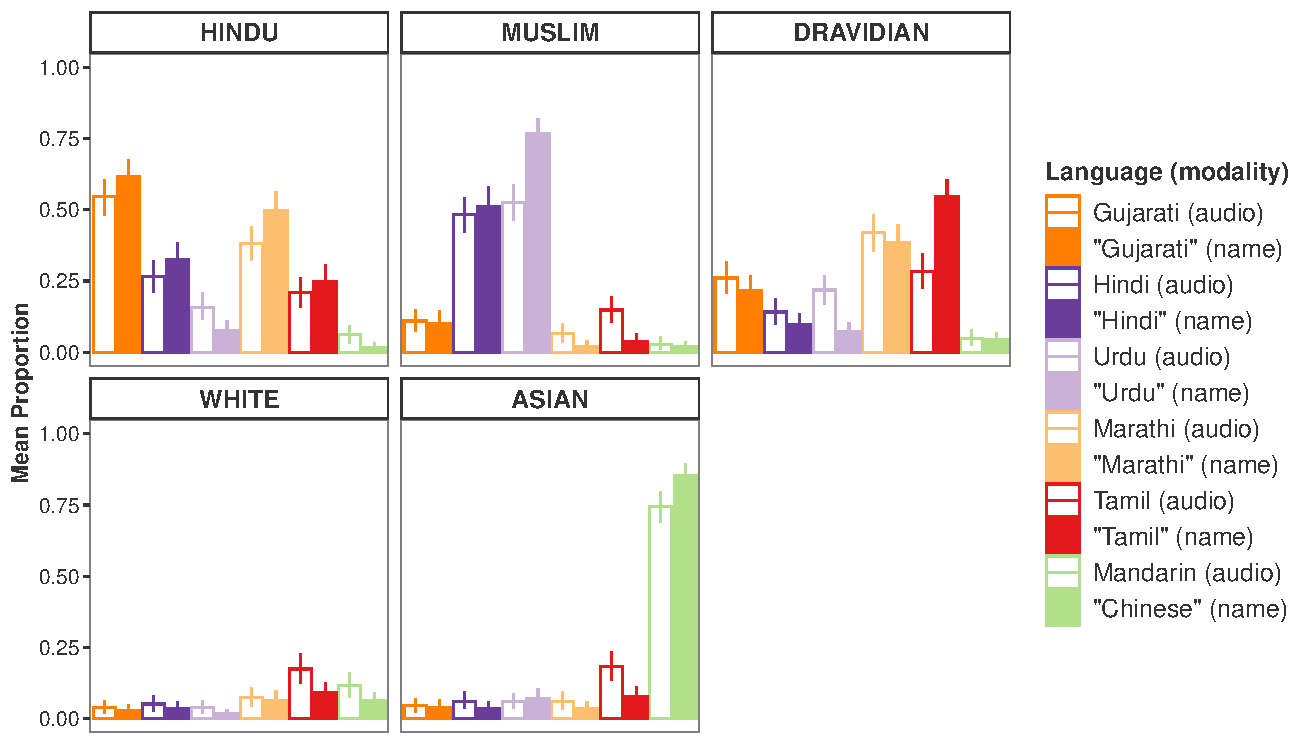
\includegraphics[width=\linewidth]{figures/plots/nonenglishes_barplot.pdf}
    \caption{\textit{Proportion of Children Selecting Each Face Type by Language and Modality.} 
    Paired bars color-coded by language reflect the mean proportion of children selecting each face type (panels), when it was presented auditorily (unfilled bars), and when it was presented by name (filled bars). 
    Error bars show 95\% bootstrapped confidence intervals.}
    \label{fig:nonenglangs}
\end{figure}
%%%% Audio vs. Language Name - English
%% latex table generated in R 4.3.2 by xtable 1.8-4 package
% Sun Jun  9 12:09:22 2024
\begin{table}[ht]
\centering
\begin{tabular}{}
  \hline
 & Predictors & Odds Ratios & CI & p & space & Odds Ratios & CI & p \\ 
  \hline
2 & langmodName: "English" & 4.33 * & 1.23 – 15.25 & 0.023 &  & 1.57 & 0.37 – 6.63 & 0.538 \\ 
  3 & langmodAudio: Indian English & 2.37 & 0.74 – 7.62 & 0.147 &  & 8.41 *** & 2.98 – 23.78 & $<$0.001 \\ 
  4 & langmodAudio: U.S. English & 1.29 & 0.58 – 2.84 & 0.534 &  & 2.70 ** & 1.34 – 5.41 & 0.005 \\ 
  5 & age & 0.87 & 0.62 – 1.24 & 0.446 &  & 0.90 & 0.65 – 1.24 & 0.501 \\ 
  6 & Observations &  &  &  &  &  &  &  \\ 
  7 & Nagelkerke's R2 &  &  &  &  &  &  &  \\ 
  8 & * p$<$0.05   ** p$<$0.01   *** p$<$0.001 &  &  &  &  &  &  &  \\ 
  21 & langmodName: "English" & 67.99 *** & 21.61 – 213.91 & $<$0.001 &  & 4.77 * & 1.37 – 16.59 & 0.014 \\ 
  31 & langmodAudio: Indian English & 38.71 *** & 14.31 – 104.72 & $<$0.001 &  & 6.92 *** & 2.42 – 19.80 & $<$0.001 \\ 
  41 & langmodAudio: U.S. English & 14.91 *** & 8.06 – 27.60 & $<$0.001 &  & 1.41 & 0.65 – 3.06 & 0.379 \\ 
  51 & age & 1.22 & 0.91 – 1.63 & 0.188 &  & 0.83 & 0.60 – 1.16 & 0.282 \\ 
  61 & Observations &  &  &  &  & 710 &  &  \\ 
  71 & Nagelkerke's R2 &  &  &  &  & 0.806 &  &  \\ 
  81 & * p$<$0.05   ** p$<$0.01   *** p$<$0.001 &  &  &  &  &  &  &  \\ 
   \hline
\end{tabular}
\end{table}

\begin{figure}[H]
    \centering
    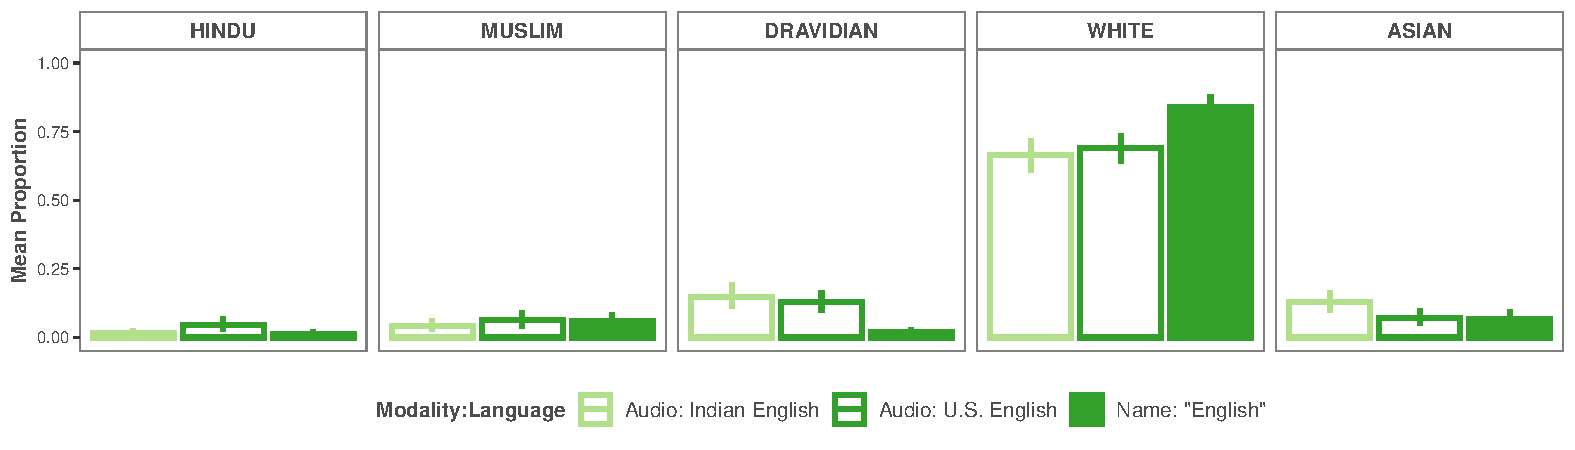
\includegraphics[width=\linewidth]{figures/plots/englishes_barplot.pdf}
    \caption{\textit{Proportion of Children Selecting Each Face Type as a Speaker of English, Probed Three Ways.} 
    Bars plot the overall proportion of children selecting each face type (panels), with error bars reflecting 95\% bootstrapped confidence intervals. Unfilled bars plot data for English variants presented auditorily (Indian English---leftmost bar, and U.S. English---middle bar), while filled bars plot mean selection data when children were asked about ``English'' by name.}    %for Three Ways of Asking About English.}  }
    \label{fig:englishes}
\end{figure}

%% ORDINAL MODELS
% latex table generated in R 4.3.2 by xtable 1.8-4 package
% Thu Jun 13 04:33:13 2024
\begin{table}[ht]
\centering
\begin{tabular}{}
  \hline
 & Predictors & Odds Ratios & CI & p \\ 
  \hline
2 & poorer$|$same & 0.23 *** & 0.17 – 0.32 & $<$0.001 \\ 
  3 & same$|$richer & 2.61 *** & 1.92 – 3.55 & $<$0.001 \\ 
  4 & language [Hindi] & 0.95 & 0.66 – 1.38 & 0.789 \\ 
  5 & language [English(India)] & 2.63 *** & 1.78 – 3.88 & $<$0.001 \\ 
  6 & language [English (U.S.)] & 2.68 *** & 1.82 – 3.93 & $<$0.001 \\ 
  7 & language [Mandarin] & 3.46 *** & 2.30 – 5.20 & $<$0.001 \\ 
  8 & language [Marathi] & 1.07 & 0.73 – 1.57 & 0.717 \\ 
  9 & language [Tamil] & 0.79 & 0.54 – 1.16 & 0.237 \\ 
  10 & language [Urdu] & 1.16 & 0.81 – 1.67 & 0.424 \\ 
  11 & child age centered & 0.88 * & 0.79 – 0.98 & 0.018 \\ 
  12 & N id & 127 &  &  \\ 
  13 & Observations & 1588 &  &  \\ 
  14 & Marginal R2 / Conditional R2 & 0.076 / 0.224 &  &  \\ 
  15 & * p$<$0.05   ** p$<$0.01   *** p$<$0.001 &  &  &  \\ 
   \hline
\end{tabular}
\end{table}

\begin{table*}[t]
\small
\caption{Cumulative Link Mixed Model of Children's Predicted Gujarati-Learning by Different Speaker Types}\label{tab:wealth-ord}
    \centering
    \vspace{5pt}
\begin{threeparttable}
\begin{tabular}{llcr}
 \toprule
& \multicolumn{3}{c}{\textbf{``\textit{Gujarati}'' Learning}\tnote{a}} \\
\cline{2-4} \\[-.75em]
\textbf{Predictors} & {OR} & {95\% CI} & \multicolumn{1}{c}{\textit{p}} \\ 
\midrule
``Not at all''$|$``Medium'' & 0.03 *** & 0.02--0.05 & $<$0.001 \\ 
``Medium''$|$``Very well'' & 0.29 *** & 0.19--0.46 & $<$0.001 \\ 
  \textsc{Muslim} & 0.22 *** & 0.12--0.40 & $<$0.001 \\ 
  \textsc{Dravidian} & 0.08 *** & 0.04--0.15 & $<$0.001 \\ 
  \textsc{White} & 0.04 *** & 0.02--0.07 & $<$0.001 \\ 
  \textsc{Asian} & 0.02 *** & 0.01--0.03 & $<$0.001 \\ 
\textsc{Hindu}:Age\tnote{b}  & 1.12 & 0.84--1.49 & 0.429 \\ 
  \textsc{Muslim}:Age & 1.09 & 0.73--1.62 & 0.678 \\ 
  \textsc{Dravidian}:Age & 0.79 & 0.52--1.18 & 0.246 \\ 
  \textsc{White}:Age & 0.60 ** & 0.41--0.87 & 0.007 \\ 
  \textsc{Asian}:Age & 0.83 & 0.55--1.26 & 0.385 \\ 
\midrule
\bfseries{\textit{N} children}\tnote{c} & 118 &  &  \\ 
\textbf{Observations}\tnote{d} & 527 &  &  \\ 
 \textbf{Marginal R2} & 0.407 &&\\
 \textbf{Conditional R2} & 0.433 &  &  \\ 
\bottomrule\\[-.75em]
\multicolumn{4}{r}{* $p<0.05$~~** $p<0.01$~~*** $p<0.001$}\\
\end{tabular}
\begin{tablenotes}[flushleft]
    \item[a] Ordinal variable: ``Very well (100\%)'' \textgreater ``Medium (50\%)'' \textgreater ``Not at all (0\%)'
    \item[b] Mean-centered, in years.
    \item[c] Model includes random intercepts for each child.
    \item[d] Model data excludes ``No opinion'' selections. 
\end{tablenotes}
\end{threeparttable}
\end{table*}

\begin{table*}[t]
\small
\caption{Cumulative Link Mixed Model of Children's Predicted English-Learning by Different Speakers}\label{tab:wealth-ord}
    \centering
    \vspace{5pt}
\begin{threeparttable}
\begin{tabular}{llcr}
 \toprule
& \multicolumn{3}{c}{\textbf{``Hindi'' Learning}\tnote{a}} \\
\cline{2-4} \\[-.75em]
\textbf{Predictors} & {OR} & {95\% CI} & \multicolumn{1}{c}{\textit{p}} \\ 
\midrule
  \hline
``Not at all''$|$``Medium'' & 0.04 *** & 0.03--0.07 & $<$0.001 \\ 
  ``Medium''$|$``Very well'' & 0.51 ** & 0.34--0.78 & 0.002 \\ 
  \textsc{Muslim} & 1.70 & 0.91--3.17 & 0.096 \\ 
  \textsc{Dravidian} & 0.32 *** & 0.18--0.57 & $<$0.001 \\ 
  \textsc{White} & 0.09 *** & 0.05--0.17 & $<$0.001 \\ 
  \textsc{Asian} & 0.05 *** & 0.03--0.10 & $<$0.001 \\ 
\textsc{Hindu}:Age\tnote{b} & 1.19 & 0.90--1.56 & 0.228 \\ 
  \textsc{Muslim}:Age & 1.13 & 0.73--1.76 & 0.583 \\ 
  \textsc{Dravidian}:Age & 0.74 & 0.50--1.08 & 0.121 \\ 
  \textsc{White}:Age & 0.63 * & 0.44--0.90 & 0.011 \\ 
  \textsc{Asian}:Age & 0.77 & 0.52--1.14 & 0.194 \\ 
\midrule
\bfseries{\textit{N} children}\tnote{c} & 118 &  &  \\ 
\textbf{Observations}\tnote{d} & 543 &  &  \\ 
 \textbf{Marginal R2} & 0.350 &  &  \\ 
 \textbf{Conditional R2}& 0.435 &  &  \\ 
 \bottomrule\\[-.75em]
\multicolumn{4}{r}{* $p<0.05$~~** $p<0.01$~~*** $p<0.001$}\\
\end{tabular}
\begin{tablenotes}[flushleft]
    \item[a] Ordinal variable: ``Very well (100\%)'' \textgreater ``Medium (50\%)'' \textgreater ``Not at all (0\%)'
    \item[b] Mean-centered, in years.
    \item[c] Model includes random intercepts for each child.
    \item[d] Model data excludes ``No opinion'' selections. 
\end{tablenotes}
\end{threeparttable}
\end{table*}

\begin{table*}[t]
\small
\caption{Cumulative Link Mixed Model of Children's Predicted Tamil-Learning by Different Speakers}\label{tab:tamil-ord}
    \centering
    \vspace{5pt}
\begin{threeparttable}
\begin{tabular}{llcr}
 \toprule
& \multicolumn{3}{c}{\textbf{``Tamil'' Learning}\tnote{a}} \\
\cline{2-4} \\[-.75em]
\textbf{Predictors} & {OR} & {95\% CI} & \multicolumn{1}{c}{\textit{p}} \\ 
\midrule
  \hline
``Not at all''$|$``Medium'' & 0.28 *** & 0.19--0.43 & $<$0.001 \\ 
``Medium''$|$``Very well'' & 2.39 *** & 1.60--3.57 & $<$0.001 \\ 
  \textsc{Muslim} & 0.29 *** & 0.17--0.50 & $<$0.001 \\ 
  \textsc{Dravidian} & 2.10 * & 1.19--3.71 & 0.010 \\ 
  \textsc{White} & 0.35 *** & 0.21--0.60 & $<$0.001 \\ 
  \textsc{Asian} & 0.40 ** & 0.23--0.70 & 0.001 \\ 
\textsc{Hindu}:Age\tnote{b}  & 0.92 & 0.72--1.17 & 0.495 \\ 
  \textsc{Muslim}:Age & 1.37 & 0.95--1.97 & 0.095 \\ 
  \textsc{Dravidian}:Age & 1.52 * & 1.03--2.25 & 0.034 \\ 
  \textsc{White}:Age & 0.70 * & 0.50--0.99 & 0.045 \\ 
  \textsc{Asian}:Age & 0.71 & 0.48--1.06 & 0.096 \\ 
\midrule
\bfseries{\textit{N} children}\tnote{c} & 117 &  &  \\ 
 \textbf{Marginal R2} & 0.190 && \\ 
 \textbf{Conditional R2} & 0.280 &  &  \\
\bottomrule\\[-.75em]
\multicolumn{4}{r}{* $p<0.05$~~** $p<0.01$~~*** $p<0.001$}\\
\end{tabular}
\begin{tablenotes}[flushleft]
    \item[a] Ordinal variable: ``Very well (100\%)'' \textgreater ``Medium (50\%)'' \textgreater ``Not at all (0\%)'
    \item[b] Mean-centered, in years.
    \item[c] Model includes random intercepts for each child.
    \item[d] Model data excludes ``No opinion'' selections. 
\end{tablenotes}
\end{threeparttable}
\end{table*}
\begin{table*}[t]
\small
\caption{Cumulative Link Mixed Model of Children's Predicted English-Learning by Different Speakers}\label{tab:english-ord}
    \centering
    \vspace{5pt}
\begin{threeparttable}
\begin{tabular}{llcr}
 \toprule
& \multicolumn{3}{c}{\textbf{``English'' Learning}\tnote{a}} \\
\cline{2-4} \\[-.75em]
\textbf{Predictors} & {OR} & {95\% CI} & \multicolumn{1}{c}{\textit{p}} \\ 
\midrule
  \hline
``Not at all''$|$``Medium'' & 0.30 *** & 0.20--0.44 & $<$0.001 \\ 
``Medium''$|$``Very well'' & 4.07 *** & 2.74--6.04 & $<$0.001 \\ 
  \textsc{Muslim} & 1.23 & 0.72--2.09 & 0.442 \\ 
  \textsc{Dravidian} & 1.38 & 0.81--2.37 & 0.241 \\ 
  \textsc{White} & 18.55 *** & 9.71--35.41 & $<$0.001 \\ 
  \textsc{Asian} & 2.20 ** & 1.26--3.85 & 0.006 \\ 
\textsc{Hindu}:Age\tnote{b} & 0.97 & 0.76--1.23 & 0.788 \\ 
  \textsc{Muslim}:Age & 1.13 & 0.78--1.64 & 0.525 \\ 
  \textsc{Dravidian}:childage centered & 0.76 & 0.53--1.10 & 0.150 \\ 
  \textsc{White}:Age & 1.42 & 0.95--2.12 & 0.088 \\ 
  \textsc{Asian}:Age & 1.38 & 0.94--2.03 & 0.102 \\ 
\midrule
\bfseries{\textit{N} children}\tnote{c} & 118 &  &  \\ 
\textbf{Observations}\tnote{d} & 519 &  &  \\ 
 \textbf{Marginal R2} & 0.300 &  &  \\ 
 \textbf{Conditional R2} & 0.308 &&\\
\bottomrule\\[-.75em]
\multicolumn{4}{r}{* $p<0.05$~~** $p<0.01$~~*** $p<0.001$}\\
\end{tabular}
\begin{tablenotes}[flushleft]
    \item[a] Ordinal variable: ``Very well (100\%)'' \textgreater ``Medium (50\%)'' \textgreater ``Not at all (0\%)'
    \item[b] Mean-centered, in years.
    \item[c] Model includes random intercepts for each child.
    \item[d] Model data excludes ``No opinion'' selections. 
\end{tablenotes}
\end{threeparttable}
\end{table*}
\begin{table*}[t]
\small
\caption{Cumulative Link Mixed Model of Children's Predicted Mandarin-Learning by Different Speakers}\label{tab:mandarin-ord}
    \centering
    \vspace{5pt}
\begin{threeparttable}
\begin{tabular}{llcr}
 \toprule
& \multicolumn{3}{c}{\textbf{``Chinese'' Learning}\tnote{a}} \\
\cline{2-4} \\[-.75em]
\textbf{Predictors} & {OR} & {95\% CI} & \multicolumn{1}{c}{\textit{p}} \\ 
\midrule
  \hline
``Not at all''$|$``Medium'' & 0.74 & 0.48--1.14 & 0.168 \\ 
``Medium''$|$``Very well'' & 13.79 *** & 7.93--23.99 & $<$0.001 \\ 
  \textsc{Muslim} & 0.68 & 0.38--1.20 & 0.183 \\ 
  \textsc{Dravidian} & 0.52 * & 0.29--0.93 & 0.028 \\ 
  \textsc{White} & 2.16 ** & 1.24--3.77 & 0.006 \\ 
  \textsc{Asian} & 146.96 *** & 58.95--366.33 & $<$0.001 \\ 
Age\tnote{b} & 1.00 & 0.84--1.18 & 0.992 \\ 
\midrule
\bfseries{\textit{N} children}\tnote{c} & 110 &  &  \\ 
\textbf{Observations}\tnote{d} & 487 &  &  \\ 
 \textbf{Marginal R2} & 0.527 &  &  \\ 
 \textbf{Conditional R2} & 0.599 &&\\
\bottomrule\\[-.75em]
\multicolumn{4}{r}{* $p<0.05$~~** $p<0.01$~~*** $p<0.001$}\\
\end{tabular}
\begin{tablenotes}[flushleft]
    \item[a] Ordinal variable: ``Very well (100\%)'' \textgreater ``Medium (50\%)'' \textgreater ``Not at all (0\%)'
    \item[b] Mean-centered, in years.
    \item[c] Model includes random intercepts for each child.
    \item[d] Model data excludes ``No opinion'' selections. 
\end{tablenotes}
\end{threeparttable}
\end{table*}

% LANGUAGE FAMILIARITY
%% Geographic origin
%% latex table generated in R 4.3.2 by xtable 1.8-4 package
% Tue Jun  4 19:27:38 2024
\begin{table*}[t]
\small
\caption{Mixed Effects Multinomial Model of Children's Geographic Origin Associations, Given Language, Child Age, and Language Familiarity}\label{tab:geoidmod}
    \centering
    \vspace{5pt}
\begin{threeparttable}
\begin{tabular}{llcrclcrc}
 \toprule
& \multicolumn{4}{c}{\textbf{Another place in India vs.}} & \multicolumn{4}{c}{\textbf{Outside India (foreign) vs.}}\\
 & \multicolumn{4}{c}{\textbf{Gujarat (same state)\tnote{a}}} & \multicolumn{4}{c}{\textbf{Gujarat (same state)\tnote{a}}}\\
\cline{2-4} \cline{6-8}\\[-.75em]
\textbf{Predictors}\tnote{b} & {OR} & {95\% CI} & \textit{p} & & {OR} & {95\% CI} & \textit{p} & \\ 
\midrule
Urdu & 0.49 *** & 0.34--0.71 & $<$0.001 &  & 0.05 *** & 0.02--0.12 & $<$0.001 \\
Marathi & 1.70 & 0.93--3.11 & 0.087 &  & 0.78 & 0.39--1.57 & 0.485 \\
Tamil & 5.25 *** & 3.10--8.90 & $<$0.001 &  & 1.69 & 0.94--3.05 & 0.081 \\
English (U.S.) & 4.58 & 0.48--43.59 & 0.186 &  & 5.06 & 0.54--47.00 & 0.154 \\
Mandarin & 4.34 ** & 1.67--11.25 & 0.003 &  & 8.74 *** & 3.60--21.21 & $<$0.001 \\
Age\tnote{c} & 1.22 ** & 1.05--1.41 & 0.008 &  & 1.18 * & 1.01--1.37 & 0.034 \\
Urdu:\textsc{Familiar} & 1.95 & 0.92--4.11 & 0.081 &  & 4.97 * & 1.42--17.44 & 0.012 \\
Marathi:\textsc{Familiar} & 0.48 & 0.17--1.38 & 0.175 &  & 0.06 *** & 0.01--0.27 & $<$0.001 \\
Tamil:\textsc{Familiar} & 0.31 * & 0.10--0.95 & 0.040 &  & 0.22 & 0.05--1.02 & 0.053 \\
English (U.S.):\textsc{Familiar} & 0.21 & 0.02--2.42 & 0.213 &  & 0.26 & 0.02--3.50 & 0.310 \\
Mandarin:\textsc{Familiar} & 0.88 & 0.16--4.86 & 0.880 &  & 0.97 & 0.14--6.64 & 0.973 \\
\midrule
\bfseries{\textit{N} children}\tnote{d} & 127 & & & & & & \\ 
\textbf{Observations}\tnote{e} & 1,127 & & & & & & & \\ 
 %& & & & & & & & \\ 
\bottomrule\\[-.75em]
\multicolumn{9}{r}{* $p<0.05$~~** $p<0.01$~~*** $p<0.001$}\\
\end{tabular}
\begin{tablenotes}[flushleft]
    \item[a] Baseline response category
    \item[b] There was insufficient variance in familiarity for Gujarati, Hindi, and Indian English to permit inclusion in this analysis. 
    \item[c] Mean-centered, in years.
    \item[d] Model includes random intercepts for each child.
    \item[e] Model data is limited to trials where children selected a geographic origin response category, i.e., excluding ``No opinion'' selections. 
\end{tablenotes}
\end{threeparttable}
\end{table*}
%% Religion
%%[\\    ]+[0-9]+ & 
%[\\    ]+[0-9]+ & 
\begin{table}[ht]
\small
\caption{Mixed Effects Multinomial Model of Children's Religious Associations, Given Language, Child Age, and Language Familiarity}
    \centering
    \vspace{5pt}
    \setlength{\tabcolsep}{1.75pt} 
\begin{threeparttable}
\begin{tabular}{lllrllllr}
\toprule
\midrule
& \multicolumn{3}{c}{\textbf{Muslim \textit{vs}.}} & & \multicolumn{3}{c}{\textbf{Jain \textit{vs}.}}\\
& \multicolumn{3}{c}{\textbf{Hindu}\tnote{a}} & & \multicolumn{3}{c}{\textbf{Hindu}\tnote{a}}\\
\cline{2-4} \cline{6-8} \\[-.75em]
\textbf{Predictors} & OR & 95\% CI & \textit{p} & & OR & 95\% CI & \textit{p} \\ 
\midrule
Gujarati & 0.19 *** & 0.11--0.35 & $<$0.001 &  & 0.18 *** & 0.09--0.36 & $<$0.001 \\ 
English (India) & 0.14 * & 0.03--0.69 & 0.016 &  & 0.62 & 0.21--1.84 & 0.391 \\ 
English (U.S.) & 0.12 & 0.01--1.48 & 0.098 &  & 0.97 & 0.07--13.77 & 0.983 \\ 
Hindi & 0.67 & 0.36--1.23 & 0.197 &  & 0.08 *** & 0.03--0.23 & $<$0.001 \\ 
Mandarin & 1.15 & 0.34--3.89 & 0.820 &  & 1.48 & 0.45--4.83 & 0.520 \\ 
Marathi & 0.12 *** & 0.07--0.19 & $<$0.001 &  & 0.35 *** & 0.22--0.57 & $<$0.001 \\ 
Tamil & 0.59 * & 0.37--0.92 & 0.019 &  & 1.28 & 0.84--1.96 & 0.251 \\ 
Urdu & 1.07 & 0.74--1.57 & 0.713 &  & 0.09 *** & 0.06--0.13 & $<$0.001 \\ 
Age\tnote{b} & 0.64 *** & 0.51--0.80 & $<$0.001 &  & 0.72 ** & 0.57--0.90 & 0.004 \\ 
Gujarati:\textsc{Familiar} & 0.64 & 0.38--1.07 & 0.090 &  & 0.24 *** & 0.13--0.45 & $<$0.001 \\ 
English (India):\textsc{Familiar} & 8.19 * & 1.30--51.76 & 0.025 &  & 8.77 ** & 2.14--35.90 & 0.003 \\ 
English (U.S.):\textsc{Familiar} & 15.69 * & 1.11--222.14 & 0.042 &  & 7.94 & 0.49--129.18 & 0.145 \\ 
Hindi:\textsc{Familiar} & 1.37 & 0.66--2.83 & 0.394 &  & 6.87 ** & 2.12--22.27 & 0.001 \\ 
Mandarin:\textsc{Familiar} & 8.27 * & 1.07--64.15 & 0.043 &  & 91.40 *** & 12.26--681.40 & $<$0.001 \\ 
Marathi:\textsc{Familiar} & 0.63 & 0.31--1.28 & 0.203 &  & 1.28 & 0.61--2.70 & 0.511 \\ 
Tamil:\textsc{Familiar} & 3.64 *** & 1.79--7.38 & $<$0.001 &  & 20.43 *** & 9.32--44.78 & $<$0.001 \\ 
Urdu:\textsc{Familiar} & 4.13 *** & 1.96--8.74 & $<$0.001 &  & 10.37 *** & 3.51--30.63 & $<$0.001 \\ 
\midrule
& \multicolumn{3}{c}{\textbf{Christian \textit{vs.}}} & &
\multicolumn{3}{c}{\textbf{Buddhist \textit{vs.}}}\\

& \multicolumn{3}{c}{\textbf{Hindu}\tnote{a}} & & \multicolumn{3}{c}{\textbf{Hindu}\tnote{a}}\\
\cline{2-4} \cline{6-8} \\[-.75em]
\textbf{Predictors} & OR & 95\% CI & \textit{p} & & OR & 95\% CI & \textit{p} \\ 
\midrule
Gujarati & 0.16 *** & 0.08--0.32 & $<$0.001 &  & 0.27 ** & 0.12--0.59 & 0.001 \\ 
English (India) & 3.00 * & 1.20--7.49 & 0.018 &  & 0.21 * & 0.06--0.79 & 0.021 \\ 
English (U.S.) & 3.20 & 0.38--26.72 & 0.283 &  & 0.87 & 0.08--9.77 & 0.909 \\ 
Hindi & 0.04 *** & 0.01--0.16 & $<$0.001 &  & 0.05 *** & 0.02--0.17 & $<$0.001 \\ 
Mandarin & 4.51 ** & 1.48--13.76 & 0.008 &  & 1.53 & 0.40--5.92 & 0.538 \\ 
Marathi & 0.23 *** & 0.14--0.36 & $<$0.001 &  & 0.53 * & 0.32--0.88 & 0.015 \\ 
Tamil & 0.84 & 0.55--1.27 & 0.400 &  & 1.22 & 0.77--1.93 & 0.396 \\ 
Urdu & 0.04 *** & 0.03--0.07 & $<$0.001 &  & 0.02 *** & 0.01--0.03 & $<$0.001 \\ 
Age\tnote{b} & 0.71 ** & 0.58--0.87 & 0.001 &  & 1.16 & 0.90--1.50 & 0.239 \\ Gujarati:\textsc{Familiar} & 0.25 *** & 0.13--0.50 & $<$0.001 &  & 0.05 *** & 0.02--0.10 & $<$0.001 \\ 
English (India):\textsc{Familiar} & 9.01 *** & 2.56--31.72 & 0.001 &  & 16.23 ** & 2.54--103.84 & 0.003 \\ 
English (U.S.):\textsc{Familiar} & 11.97 * & 1.21--118.02 & 0.033 &  & 22.50 * & 1.65--305.96 & 0.019 \\ 
Hindi:\textsc{Familiar} & 3.46 & 0.66--18.21 & 0.143 &  & 6.31 ** & 1.65--24.18 & 0.007 \\ 
Mandarin:\textsc{Familiar} & 32.64 *** & 4.53--235.08 & 0.001 &  & 201.38 *** & 23.29--1741.37 & $<$0.001 \\ 
Marathi:\textsc{Familiar} & 0.91 & 0.38--2.14 & 0.823 &  & 2.48 * & 1.05--5.88 & 0.039 \\ 
Tamil:\textsc{Familiar} & 8.28 *** & 3.45--19.85 & $<$0.001 &  & 47.12 *** & 19.03--116.64 & $<$0.001 \\ 
Urdu:\textsc{Familiar} & 8.68 ** & 2.20--34.29 & 0.002 &  & 51.96 *** & 11.41--236.57 & $<$0.001 \\ 
\midrule
\bfseries{\textit{N} children}\tnote{c} & 129&   &  &  &  &  \\
\textbf{Observations}\tnote{d} & 1,580  &  &  &  &  &  &  \\
\bottomrule
\multicolumn{8}{r}{* $p<0.05$~~** $p<0.01$~~*** $p<0.001$}\\
\end{tabular}
\begin{tablenotes}[flushleft]
    \item[a] Baseline response category selected on 31\% of religious association trials, by 129 children. % (574/1856)
    \item[b] Mean-centered, in years.
    \item[c] Model includes random intercepts for each child.
    \item[d] Model data is limited to trials where children selected a single religion, i.e., excluding selections of multiple religions or ``No opinion.'' 
\end{tablenotes}
\end{threeparttable}
\end{table}
%% Face-audio
%% latex table generated in R 4.3.2 by xtable 1.8-4 package
% Thu Jun 13 04:39:33 2024
\begin{table}[ht]
\centering
\begin{tabular}{}
  \hline
 & Predictors & Odds Ratios & CI & p & space & Odds Ratios & CI & p \\ 
  \hline
2 & Gujarati & 2.55 & 0.27 – 23.89 & 0.413 &  & 3.07 & 0.31 – 30.76 & 0.339 \\ 
  3 & Urdu & 3.06 *** & 1.98 – 4.72 & $<$0.001 &  & 1.31 & 0.80 – 2.15 & 0.278 \\ 
  4 & Marathi & 0.27 ** & 0.11 – 0.64 & 0.003 &  & 1.73 & 0.99 – 3.02 & 0.054 \\ 
  5 & Tamil & 0.85 & 0.49 – 1.48 & 0.572 &  & 1.39 & 0.85 – 2.26 & 0.187 \\ 
  6 & English (U.S.) & 0.92 & 0.00 – Inf & 1.000 &  & 117444098584.75 & 0.00 – Inf & 1.000 \\ 
  7 & Mandarin & 0.45 & 0.13 – 1.50 & 0.192 &  & 0.99 & 0.37 – 2.65 & 0.977 \\ 
  8 & familiar & 0.06 * & 0.01 – 0.63 & 0.019 &  & 0.15 & 0.01 – 1.51 & 0.107 \\ 
  9 & age & 0.79 *** & 0.69 – 0.90 & 0.001 &  & 1.00 & 0.89 – 1.12 & 0.988 \\ 
  10 & Urdu:familiar & 22.20 * & 1.90 – 259.18 & 0.013 &  & 8.22 & 0.65 – 104.53 & 0.104 \\ 
  11 & Marathi:familiar & 7.38 & 0.58 – 93.73 & 0.123 &  & 3.71 & 0.33 – 41.17 & 0.285 \\ 
  12 & Tamil:familiar & 8.10 & 0.68 – 97.00 & 0.099 &  & 6.26 & 0.54 – 72.95 & 0.143 \\ 
  13 & English (U.S.):familiar & 40.79 & 0.00 – Inf & 1.000 &  & 0.00 & 0.00 – Inf & 1.000 \\ 
  14 & Mandarin:familiar & 12.52 & 0.60 – 259.69 & 0.102 &  & 3.45 & 0.19 – 61.29 & 0.398 \\ 
  15 & N id &  &  &  &  &  &  &  \\ 
  16 & Observations &  &  &  &  &  &  &  \\ 
  17 & * p$<$0.05   ** p$<$0.01   *** p$<$0.001 &  &  &  &  &  &  &  \\ 
  21 & Gujarati & 0.95 & 0.06 – 15.69 & 0.969 &  & 0.00 & 0.00 – Inf & 1.000 \\ 
  31 & Urdu & 0.28 ** & 0.13 – 0.62 & 0.002 &  & 0.46 * & 0.24 – 0.90 & 0.023 \\ 
  41 & Marathi & 0.42 * & 0.19 – 0.92 & 0.031 &  & 0.32 ** & 0.14 – 0.74 & 0.008 \\ 
  51 & Tamil & 0.94 & 0.55 – 1.61 & 0.829 &  & 1.01 & 0.60 – 1.71 & 0.964 \\ 
  61 & English (U.S.) & 400714652877.87 & 0.00 – Inf & 1.000 &  & 221042843443.43 & 0.00 – Inf & 1.000 \\ 
  71 & Mandarin & 1.44 & 0.58 – 3.56 & 0.427 &  & 5.21 *** & 2.43 – 11.18 & $<$0.001 \\ 
  81 & familiar & 0.07 & 0.00 – 1.19 & 0.065 &  & 8856110008.68 & 0.00 – Inf & 1.000 \\ 
  91 & age & 0.95 & 0.83 – 1.09 & 0.449 &  & 0.85 * & 0.74 – 0.98 & 0.021 \\ 
  101 & Urdu:familiar & 6.79 & 0.17 – 263.99 & 0.305 &  & 0.00 & 0.00 – Inf & 1.000 \\ 
  111 & Marathi:familiar & 4.59 & 0.21 – 100.23 & 0.332 &  & 0.00 & 0.00 – Inf & 1.000 \\ 
  121 & Tamil:familiar & 10.91 & 0.52 – 227.27 & 0.123 &  & 0.00 & 0.00 – Inf & 1.000 \\ 
  131 & English (U.S.):familiar & 0.00 & 0.00 – Inf & 1.000 &  & 0.00 & 0.00 – Inf & 1.000 \\ 
  141 & Mandarin:familiar & 25.67 * & 1.07 – 614.54 & 0.045 &  & 0.00 & 0.00 – Inf & 1.000 \\ 
  151 & N id &  &  &  &  & 126 &  &  \\ 
  161 & Observations &  &  &  &  & 1390 &  &  \\ 
  171 & * p$<$0.05   ** p$<$0.01   *** p$<$0.001 &  &  &  &  &  &  &  \\ 
   \hline
\end{tabular}
\end{table}

%% Face-label
%% latex table generated in R 4.3.2 by xtable 1.8-4 package
% Mon Jun 10 14:35:24 2024
\begin{table}[ht]
\centering
\begin{tabular}{}
  \hline
 & Predictors & Odds Ratios & CI & p & space & Odds Ratios & CI & p \\ 
  \hline
2 & Gujarati & 0.61 & 0.05 – 6.84 & 0.687 &  & 0.48 & 0.04 – 5.30 & 0.546 \\ 
  3 & Urdu & 8.44 *** & 4.94 – 14.42 & $<$0.001 &  & 1.00 & 0.49 – 2.04 & 0.998 \\ 
  4 & Marathi & 0.04 ** & 0.01 – 0.31 & 0.002 &  & 1.61 & 0.97 – 2.66 & 0.064 \\ 
  5 & Tamil & 0.18 *** & 0.08 – 0.41 & $<$0.001 &  & 2.26 *** & 1.53 – 3.34 & $<$0.001 \\ 
  6 & Mandarin & 0.66 & 0.11 – 3.97 & 0.652 &  & 3.66 * & 1.02 – 13.11 & 0.047 \\ 
  7 & familiar & 0.26 & 0.02 – 3.06 & 0.284 &  & 0.74 & 0.06 – 8.39 & 0.805 \\ 
  8 & age & 1.10 & 0.95 – 1.29 & 0.203 &  & 0.98 & 0.88 – 1.08 & 0.648 \\ 
  9 & Urdu:familiar & 8.78 & 0.54 – 142.96 & 0.127 &  & 0.89 & 0.04 – 20.01 & 0.944 \\ 
  10 & Marathi:familiar & 3.76 & 0.14 – 103.66 & 0.434 &  & 0.46 & 0.04 – 5.59 & 0.541 \\ 
  11 & Tamil:familiar & 1.95 & 0.10 – 38.42 & 0.662 &  & 1.28 & 0.10 – 15.89 & 0.848 \\ 
  12 & Mandarin:familiar & 16.23 & 0.37 – 718.25 & 0.149 &  & 0.00 & 0.00 – Inf & 1.000 \\ 
  13 & N id &  &  &  &  &  &  &  \\ 
  14 & Observations &  &  &  &  &  &  &  \\ 
  15 & * p$<$0.05   ** p$<$0.01   *** p$<$0.001 &  &  &  &  &  &  &  \\ 
  21 & Gujarati & 0.23 & 0.02 – 2.62 & 0.235 &  & 1.49 & 0.26 – 8.45 & 0.651 \\ 
  31 & Urdu & 0.17 ** & 0.05 – 0.59 & 0.006 &  & 1.10 & 0.55 – 2.22 & 0.780 \\ 
  41 & Marathi & 0.21 *** & 0.09 – 0.49 & $<$0.001 &  & 0.18 *** & 0.07 – 0.47 & $<$0.001 \\ 
  51 & Tamil & 0.45 ** & 0.25 – 0.81 & 0.008 &  & 0.28 *** & 0.14 – 0.56 & $<$0.001 \\ 
  61 & Mandarin & 2.13 & 0.55 – 8.18 & 0.272 &  & 19.82 *** & 6.21 – 63.25 & $<$0.001 \\ 
  71 & familiar & 0.14 & 0.01 – 1.82 & 0.132 &  & 0.02 *** & 0.00 – 0.17 & $<$0.001 \\ 
  81 & age & 0.69 *** & 0.58 – 0.84 & $<$0.001 &  & 0.87 & 0.74 – 1.02 & 0.093 \\ 
  91 & Urdu:familiar & 9.87 & 0.25 – 385.47 & 0.221 &  & 0.00 & 0.00 – Inf & 1.000 \\ 
  101 & Marathi:familiar & 2.65 & 0.16 – 43.78 & 0.495 &  & 8.13 & 0.71 – 93.17 & 0.092 \\ 
  111 & Tamil:familiar & 2.47 & 0.14 – 43.03 & 0.535 &  & 53.04 *** & 5.72 – 491.88 & $<$0.001 \\ 
  121 & Mandarin:familiar & 25.89 & 0.72 – 925.72 & 0.075 &  & 321.53 *** & 16.19 – 6386.79 & $<$0.001 \\ 
  131 & N id &  &  &  &  & 126 &  &  \\ 
  141 & Observations &  &  &  &  & 1178 &  &  \\ 
  151 & * p$<$0.05   ** p$<$0.01   *** p$<$0.001 &  &  &  &  &  &  &  \\ 
   \hline
\end{tabular}
\end{table}


%% GENDER
%\begin{table*}[t]
\small
\caption{Mixed Effects Multinomial Model of Children's Geographic Origin Associations, Given Language, Child Age, and Speaker Gender}\label{tab:geo-gender-mod}
    \centering
    \vspace{5pt}
\begin{threeparttable}
\begin{tabular}{llcrclcrc}
 \toprule
  & \multicolumn{4}{c}{\textbf{Another place in India vs.}} & \multicolumn{4}{c}{\textbf{Outside India (foreign) vs.}}\\
 & \multicolumn{4}{c}{\textbf{Gujarat (same state)\tnote{a}}} & \multicolumn{4}{c}{\textbf{Gujarat (same state)\tnote{a}}}\\
\cline{2-4} \cline{6-8}\\[-.75em]
\textbf{Predictors} & {OR} & {95\% CI} & \multicolumn{1}{c}{\textit{p}} & & {OR} & {95\% CI} & \multicolumn{1}{c}{\textit{p}} & \\ 
\midrule
 Gujarati & 0.31 *** & 0.19--0.51 & $<$0.001 &  & 0.31 *** & 0.19--0.52 & $<$0.001 \\ 
 Hindi & 0.71 & 0.47--1.05 & 0.087 &  & 0.03 *** & 0.01--0.14 & $<$0.001 \\ 
 Urdu & 0.92 & 0.61--1.37 & 0.666 &  & 0.08 *** & 0.03--0.22 & $<$0.001 \\ 
 Marathi & 1.45 & 0.95--2.20 & 0.082 &  & 0.27 *** & 0.13--0.54 & $<$0.001 \\ 
 Tamil & 4.16 *** & 2.41--7.18 & $<$0.001 &  & 1.12 & 0.57--2.19 & 0.748 \\ 
 English (India) & 1.42 & 0.66--3.06 & 0.372 &  & 6.49 *** & 3.44--12.25 & $<$0.001 \\ 
 English (U.S.) & 2.81 ** & 1.32--6.01 & 0.008 &  & 7.38 *** & 3.68--14.81 & $<$0.001 \\ 
 Mandarin & 4.53 * & 1.30--15.78 & 0.018 &  & 27.06 *** & 8.54--85.68 & $<$0.001 \\ 
 Age\tnote{b} & 1.07 & 0.98--1.16 & 0.125 &  & 1.03 & 0.93--1.13 & 0.624 \\ 
 Gujarati:\textsc{Female} & 0.58 & 0.28--1.20 & 0.142 &  & 0.20 ** & 0.08--0.54 & 0.001 \\ 
 Hindi:\textsc{Female} & 1.06 & 0.42--2.66 & 0.898 &  & 9.28 * & 1.34--64.16 & 0.024 \\ 
 Urdu:\textsc{Female} & 0.82 & 0.32--2.05 & 0.663 &  & 5.75 * & 1.16--28.57 & 0.033 \\ 
 Marathi:\textsc{Female} & 2.21 & 0.87--5.60 & 0.094 &  & 6.77 ** & 1.75--26.18 & 0.006 \\ 
 Tamil:\textsc{Female} & 2.09 & 0.71--6.17 & 0.182 &  & 10.80 *** & 2.82--41.36 & 0.001 \\ 
 English (India):\textsc{Female} & 1.48 & 0.44--4.91 & 0.524 &  & 2.51 & 0.71--8.79 & 0.151 \\ 
 English (U.S.):\textsc{Female} & 0.98 & 0.28--3.42 & 0.970 &  & 4.08 * & 1.08--15.37 & 0.038 \\ 
 Mandarin:\textsc{Female} & 2.72 & 0.46--16.11 & 0.271 &  & 3.56 & 0.58--21.75 & 0.168 \\ 
\midrule
\textbf{Observations}\tnote{c} & 1,725 & & & & & & & \\ 
\textbf{Nagelkerke's R2} & 0.492 & & & & & & & \\ 
\bottomrule\\[-.75em]
\multicolumn{9}{r}{* $p<0.05$~~** $p<0.01$~~*** $p<0.001$}\\
\end{tabular}
\begin{tablenotes}[flushleft]
    \item[a] Baseline response category selected on 33\% of geographic origin association trials, by 127 children. % (606/1834)
    \item[b] Mean-centered, in years.
    \item[c] Model data is limited to trials where children selected a geographic origin response category, i.e., excluding ``No opinion'' selections. 
\end{tablenotes}
\end{threeparttable}
\end{table*}
%\begin{table}[ht]
\small
\caption{Mixed Effects Multinomial Model of Children's Religious Associations, Given Language, Child Age, and Speaker Gender}\label{tab:rel-gender-mod}
    \centering
    \vspace{5pt}
    \setlength{\tabcolsep}{1.75pt} 
\begin{threeparttable}
\begin{tabular}{lllllllll}
\toprule
\midrule
& \multicolumn{3}{c}{\textbf{Muslim \textit{vs}.}} & & \multicolumn{3}{c}{\textbf{Jain \textit{vs}.}}\\
& \multicolumn{3}{c}{\textbf{Hindu}\tnote{a}} & & \multicolumn{3}{c}{\textbf{Hindu}\tnote{a}}\\
\cline{2-4} \cline{6-8} \\[-.75em]
\textbf{Predictors} & OR & 95\% CI & \multicolumn{1}{c}{\textit{p}} & & OR & 95\% CI & \multicolumn{1}{c}{\textit{p}} \\ 
\midrule
 Gujarati & 0.23 *** & 0.13--0.42 & $<$0.001 &  & 0.16 *** & 0.08--0.32 & $<$0.001 \\ 
 English (India) & 0.77 & 0.27--2.22 & 0.628 &  & 1.80 & 0.76--4.31 & 0.184 \\ 
 English (U.S.) & 0.80 & 0.31--2.03 & 0.637 &  & 1.11 & 0.47--2.63 & 0.805 \\ 
 Hindi & 0.77 & 0.50--1.20 & 0.252 &  & 0.24 *** & 0.12--0.46 & $<$0.001 \\ 
 Mandarin & 4.76 * & 1.02--22.09 & 0.046 &  & 6.84 * & 1.54--30.35 & 0.011 \\ 
 Marathi & 0.07 *** & 0.03--0.20 & $<$0.001 &  & 0.27 *** & 0.15--0.48 & $<$0.001 \\ 
 Tamil & 0.57 & 0.27--1.19 & 0.134 &  & 1.09 & 0.59--2.01 & 0.790 \\ 
 Urdu & 1.44 & 0.94--2.22 & 0.093 &  & 0.20 *** & 0.09--0.45 & $<$0.001 \\ 
 Age\tnote{b} & 0.79 *** & 0.71--0.87 & $<$0.001 &  & 0.85 ** & 0.76--0.96 & 0.006 \\ 
 Gujarati:\textsc{Female} & 0.57 & 0.24--1.35 & 0.200 &  & 0.63 & 0.24--1.69 & 0.360 \\ 
 English (India):\textsc{Female} & 0.92 & 0.19--4.32 & 0.911 &  & 0.47 & 0.11--2.06 & 0.317 \\ 
 English (U.S.):\textsc{Female} & 3.60 & 0.75--17.40 & 0.111 &  & 3.80 & 0.79--18.23 & 0.095 \\ 
 Hindi:\textsc{Female} & 1.39 & 0.49--3.95 & 0.536 &  & 0.94 & 0.24--3.71 & 0.931 \\ 
 Mandarin:\textsc{Female} & 0.77 & 0.09--6.38 & 0.806 &  & 1.17 & 0.15--9.41 & 0.880 \\ 
 Marathi:\textsc{Female} & 6.33 * & 1.48--27.14 & 0.013 &  & 1.33 & 0.36--4.86 & 0.669 \\ 
 Tamil:\textsc{Female} & 3.19 & 0.83--12.29 & 0.091 &  & 3.20 & 0.85--11.99 & 0.084 \\ 
 Urdu:\textsc{Female} & 0.91 & 0.32--2.57 & 0.865 &  & 0.82 & 0.18--3.78 & 0.803 \\ 
\midrule
& \multicolumn{3}{c}{\textbf{Christian vs.}} & &
\multicolumn{3}{c}{\textbf{Buddhist vs.}}\\

& \multicolumn{3}{c}{\textbf{Hindu}\tnote{a}} & & \multicolumn{3}{c}{\textbf{Hindu}\tnote{a}}\\
\cline{2-4} \cline{6-8} \\[-.75em]
\textbf{Predictors} & OR & 95\% CI & \multicolumn{1}{c}{\textit{p}} & & OR & 95\% CI & \multicolumn{1}{c}{\textit{p}} \\ 
\midrule
 Gujarati & 0.13 *** & 0.06--0.28 & $<$0.001 &  & 0.11 *** & 0.05--0.25 & $<$0.001 \\ 
 English (India) & 5.45 *** & 2.56--11.59 & $<$0.001 &  & 0.47 & 0.14--1.58 & 0.225 \\ 
 English (U.S.) & 3.97 *** & 1.98--7.95 & $<$0.001 &  & 1.06 & 0.45--2.49 & 0.900 \\ 
 Hindi & 0.08 *** & 0.03--0.22 & $<$0.001 &  & 0.04 *** & 0.01--0.16 & $<$0.001 \\ 
 Mandarin & 12.35 *** & 2.92--52.19 & 0.001 &  & 6.10 * & 1.37--27.12 & 0.017 \\ 
 Marathi & 0.10 *** & 0.04--0.24 & $<$0.001 &  & 0.23 *** & 0.13--0.42 & $<$0.001 \\ 
 Tamil & 0.45 * & 0.20--0.98 & 0.044 &  & 1.61 & 0.92--2.82 & 0.092 \\ 
 Urdu & 0.03 *** & 0.00--0.19 & $<$0.001 &  & 0.07 *** & 0.02--0.24 & $<$0.001 \\ 
 Age\tnote{b} & 1.02 & 0.91--1.15 & 0.682 &  & 1.11 & 0.97--1.27 & 0.123 \\ 
 Gujarati:\textsc{Female} & 0.25 * & 0.06--0.97 & 0.045 &  & 0.19 * & 0.04--0.95 & 0.044 \\
 English (India):\textsc{Female} & 1.39 & 0.27--7.14 & 0.695 &  & 3.13 & 0.36--27.51 & 0.304 \\ 
 English (U.S.):\textsc{Female} & 6.82 * & 1.21--38.31 & 0.029 &  & 6.21 & 0.78--49.26 & 0.084 \\ 
 Hindi:\textsc{Female} & 0.77 & 0.06--10.42 & 0.842 &  & 2.01 & 0.11--37.04 & 0.638 \\ 
 Mandarin:\textsc{Female} & 1.88 & 0.20--17.92 & 0.581 &  & 3.60 & 0.31--41.58 & 0.305 \\ 
 Marathi:\textsc{Female} & 7.28 * & 1.28--41.54 & 0.025 &  & 5.30 & 0.86--32.51 & 0.072 \\ 
 Tamil:\textsc{Female} & 10.34 ** & 1.83--58.47 & 0.008 &  & 3.37 & 0.53--21.43 & 0.197 \\ 
 Urdu:\textsc{Female} & 10.31 & 0.75--140.88 & 0.080 &  & 1.13 & 0.07--18.69 & 0.932 \\ 
 \midrule
\textbf{Observations}\tnote{c} & 1,511  &  &  &  &  &  &  \\
\textbf{Nagelkerke's R2} & 0.567  &  &  &  &  &  &  \\
\bottomrule
\multicolumn{8}{r}{* $p<0.05$~~** $p<0.01$~~*** $p<0.001$}\\
\end{tabular}
\begin{tablenotes}[flushleft]
    \item[a] Baseline response category selected on 31\% of religious association trials, by 129 children. % (574/1856)
    \item[b] Mean-centered, in years.
    \item[c] Model data is limited to trials where children selected a single religion, i.e., excluding selections of multiple religions or ``No opinion.'' 
\end{tablenotes}
\end{threeparttable}
\end{table}

%\begin{table*}[t]
\small
\caption{Cumulative Link Mixed Model of Children's Wealth Associations, Given Language, Child Age, and Speaker Gender}\label{tab:wealth-gender-ord}
    \centering
    \vspace{5pt}
\begin{threeparttable}
\begin{tabular}{llcr}
 \toprule
& \multicolumn{3}{c}{\textbf{Wealth}\tnote{a}} \\
\cline{2-4} \\[-.75em]
\textbf{Predictors} & {OR} & {95\% CI} & \multicolumn{1}{c}{\textit{p}} \\ 
\midrule
``less money''$|$``as much money'' & 0.19 *** & 0.13--0.30 & $<$0.001 \\ 
  ``as much money''$|$``more money'' & 2.19 *** & 1.43--3.34 & $<$0.001 \\ 
  Hindi & 1.01 & 0.58--1.75 & 0.970 \\ 
  English(India) & 2.20 ** & 1.23--3.96 & 0.008 \\ 
  English (U.S.) & 1.80 * & 1.04--3.12 & 0.037 \\
  Mandarin & 4.46 *** & 2.44--8.13 & $<$0.001 \\ 
  Marathi & 1.09 & 0.62--1.91 & 0.759 \\ 
  Tamil & 0.58 & 0.33--1.03 & 0.061 \\ 
  Urdu & 1.05 & 0.61--1.80 & 0.868 \\ 
  Age\tnote{b} & 0.87 * & 0.77--0.98 & 0.021 \\ 
  Gujarati:\textsc{Female} & 0.67 & 0.39--1.15 & 0.150 \\ 
  Hindi:\textsc{Female} & 1.03 & 0.48--2.21 & 0.933 \\ 
  English(India):\textsc{Female} & 1.54 & 0.69--3.42 & 0.288 \\ 
  English (U.S.):\textsc{Female} & 2.67 * & 1.21--5.86 & 0.014 \\
  Mandarin:\textsc{Female} & 0.63 & 0.28--1.45 & 0.277 \\ 
  Marathi:\textsc{Female} & 1.02 & 0.46--2.22 & 0.969 \\ 
  Tamil:\textsc{Female} & 1.81 & 0.83--3.94 & 0.136 \\ 
  Urdu:\textsc{Female} & 1.31 & 0.62--2.77 & 0.474 \\ 
\midrule
\bfseries{\textit{N} children}\tnote{c} & 127 & & \\ 
\textbf{Observations}\tnote{d} & 1,588 & &\\ 
 \textbf{Marginal R2} &  0.092 &&\\
 \textbf{Conditional R2} & 0.245 &  &  \\ 
\bottomrule\\[-.75em]
\multicolumn{4}{r}{* $p<0.05$~~** $p<0.01$~~*** $p<0.001$}\\
\end{tabular}
\begin{tablenotes}[flushleft]
    \item[a] Ordinal variable: ``more money than the people in my city'' \textgreater ``as much money as the people in my city'' \textgreater ``less money than the people in my city''
    \item[b] Mean-centered, in years.
    \item[c] Model includes random intercepts for each child.
    \item[d] Model data excludes ``No opinion'' selections. 
\end{tablenotes}
\end{threeparttable}
\end{table*}
%% latex table generated in R 4.3.2 by xtable 1.8-4 package
% Thu Jun 13 04:39:43 2024
\begin{table}[ht]
\centering
\begin{tabular}{}
  \hline
 & Predictors & Odds Ratios & CI & p & space & Odds Ratios & CI & p \\ 
  \hline
2 & Gujarati & 0.16 *** & 0.09 – 0.31 & $<$0.001 &  & 0.40 *** & 0.25 – 0.63 & $<$0.001 \\ 
  3 & Hindi & 1.33 & 0.86 – 2.07 & 0.202 &  & 0.36 ** & 0.19 – 0.69 & 0.002 \\ 
  4 & Urdu & 3.79 *** & 2.27 – 6.34 & $<$0.001 &  & 0.48 & 0.21 – 1.06 & 0.068 \\ 
  5 & Marathi & 0.19 *** & 0.09 – 0.39 & $<$0.001 &  & 0.82 & 0.53 – 1.27 & 0.382 \\ 
  6 & Tamil & 1.10 & 0.58 – 2.05 & 0.775 &  & 2.01 * & 1.15 – 3.51 & 0.014 \\ 
  7 & English (India) & 0.37 & 0.10 – 1.40 & 0.142 &  & 2.38 * & 1.04 – 5.46 & 0.041 \\ 
  8 & English (U.S.) & 3.95 & 0.84 – 18.67 & 0.083 &  & 13.57 *** & 3.22 – 57.20 & $<$0.001 \\ 
  9 & Mandarin & 0.51 & 0.13 – 2.06 & 0.347 &  & 1.02 & 0.33 – 3.16 & 0.977 \\ 
  10 & speaker\_FEMALE & 1.40 & 0.60 – 3.30 & 0.436 &  & 1.38 & 0.74 – 2.55 & 0.309 \\ 
  11 & age & 0.87 * & 0.78 – 0.97 & 0.011 &  & 0.97 & 0.88 – 1.08 & 0.589 \\ 
  12 & Hindi:speaker\_FEMALE & 1.30 & 0.45 – 3.78 & 0.624 &  & 1.55 & 0.54 – 4.48 & 0.416 \\ 
  13 & Urdu:speaker\_FEMALE & 0.53 & 0.17 – 1.64 & 0.269 &  & 3.52 * & 1.12 – 11.08 & 0.032 \\ 
  14 & Marathi:speaker\_FEMALE & 0.54 & 0.13 – 2.20 & 0.389 &  & 1.28 & 0.55 – 2.99 & 0.574 \\ 
  15 & Tamil:speaker\_FEMALE & 0.29 & 0.08 – 1.01 & 0.052 &  & 0.33 * & 0.12 – 0.87 & 0.025 \\ 
  16 & English (India):speaker\_FEMALE & 11.57 * & 1.31 – 102.04 & 0.027 &  & 1.69 & 0.27 – 10.49 & 0.573 \\ 
  17 & English (U.S.):speaker\_FEMALE & 0.18 & 0.01 – 2.53 & 0.204 &  & 0.22 & 0.02 – 1.96 & 0.173 \\ 
  18 & Mandarin:speaker\_FEMALE & 0.54 & 0.07 – 4.38 & 0.561 &  & 0.45 & 0.08 – 2.49 & 0.362 \\ 
  19 & N id &  &  &  &  &  &  &  \\ 
  20 & Observations &  &  &  &  &  &  &  \\ 
  21 & * p$<$0.05   ** p$<$0.01   *** p$<$0.001 &  &  &  &  &  &  &  \\ 
  22 & Gujarati & 0.11 *** & 0.05 – 0.23 & $<$0.001 &  & 0.12 *** & 0.06 – 0.25 & $<$0.001 \\ 
  31 & Hindi & 0.28 *** & 0.14 – 0.56 & $<$0.001 &  & 0.22 *** & 0.10 – 0.48 & $<$0.001 \\ 
  41 & Urdu & 0.37 * & 0.15 – 0.88 & 0.025 &  & 0.31 * & 0.12 – 0.79 & 0.014 \\ 
  51 & Marathi & 0.28 *** & 0.15 – 0.52 & $<$0.001 &  & 0.15 *** & 0.07 – 0.33 & $<$0.001 \\ 
  61 & Tamil & 0.69 & 0.34 – 1.40 & 0.299 &  & 1.20 & 0.65 – 2.22 & 0.564 \\ 
  71 & English (India) & 9.53 *** & 4.58 – 19.82 & $<$0.001 &  & 1.35 & 0.54 – 3.37 & 0.522 \\ 
  81 & English (U.S.) & 30.57 *** & 7.46 – 125.31 & $<$0.001 &  & 9.38 ** & 2.18 – 40.40 & 0.003 \\ 
  91 & Mandarin & 1.85 & 0.68 – 5.03 & 0.225 &  & 13.73 *** & 5.96 – 31.65 & $<$0.001 \\ 
  101 & speaker\_FEMALE & 0.29 & 0.06 – 1.46 & 0.135 &  & 0.39 & 0.10 – 1.52 & 0.174 \\ 
  111 & age & 0.95 & 0.85 – 1.07 & 0.437 &  & 0.85 ** & 0.75 – 0.95 & 0.006 \\ 
  121 & Hindi:speaker\_FEMALE & 0.95 & 0.10 – 9.22 & 0.967 &  & 2.71 & 0.44 – 16.53 & 0.279 \\ 
  131 & Urdu:speaker\_FEMALE & 1.04 & 0.10 – 10.80 & 0.974 &  & 3.70 & 0.58 – 23.59 & 0.166 \\ 
  141 & Marathi:speaker\_FEMALE & 1.19 & 0.16 – 8.85 & 0.865 &  & 2.95 & 0.50 – 17.48 & 0.234 \\ 
  151 & Tamil:speaker\_FEMALE & 4.50 & 0.72 – 28.23 & 0.108 &  & 1.42 & 0.28 – 7.09 & 0.673 \\ 
  161 & English (India):speaker\_FEMALE & 15.96 * & 1.67 – 152.32 & 0.016 &  & 5.72 & 0.57 – 56.98 & 0.137 \\ 
  171 & English (U.S.):speaker\_FEMALE & 5.27 & 0.41 – 68.04 & 0.202 &  & 1.52 & 0.12 – 18.64 & 0.744 \\ 
  181 & Mandarin:speaker\_FEMALE & 3.51 & 0.44 – 28.04 & 0.236 &  & 2.10 & 0.36 – 12.26 & 0.408 \\ 
  191 & N id &  &  &  &  & 126 &  &  \\ 
  201 & Observations &  &  &  &  & 1849 &  &  \\ 
  211 & * p$<$0.05   ** p$<$0.01   *** p$<$0.001 &  &  &  &  &  &  &  \\ 
   \hline
\end{tabular}
\end{table}

%% latex table generated in R 4.3.2 by xtable 1.8-4 package
% Tue Jun  4 19:00:35 2024
%[\\    ]+[0-9]+ & 
%[\\    ]+[0-9]+ & 
\begin{table}[ht]
\small
\caption{Mixed Effects Multinomial Model of Children's Single-Face Selection for Languages Presented by Name, Given Language, Child Age, and Speaker Gender}\label{tab:fl-gen-mod}
    \centering
    \vspace{5pt}
    \setlength{\tabcolsep}{1.75pt} 
\begin{threeparttable}
\begin{tabular}{lllrllllr}
\toprule
& \multicolumn{3}{c}{\textbf{Muslim vs.}} & & \multicolumn{3}{c}{\textbf{South Indian Hindu vs.}}\\
& \multicolumn{3}{c}{\textbf{North Indian Hindu}\tnote{a}} & & \multicolumn{3}{c}{\textbf{North Indian Hindu}\tnote{a}}\\
\cline{2-4} \cline{6-8} \\[-.75em]
\textbf{Predictors} & OR & 95\% CI & \multicolumn{1}{c}{\textit{p}} & & OR & 95\% CI & \multicolumn{1}{c}{\textit{p}} \\ 
\midrule
Gujarati & 0.14 *** & 0.07--0.27 & $<$0.001 &  & 0.18 *** & 0.10--0.31 & $<$0.001 \\ 
  Hindi & 0.72 & 0.47--1.11 & 0.137 &  & 0.28 *** & 0.15--0.50 & $<$0.001 \\ 
  Urdu & 10.76 *** & 5.20--22.24 & $<$0.001 &  & 1.49 & 0.61--3.66 & 0.379 \\ 
  Marathi & 0.06 *** & 0.02--0.18 & $<$0.001 &  & 0.74 & 0.49--1.12 & 0.153 \\ 
  Tamil & 0.37 * & 0.15--0.88 & 0.024 &  & 3.52 *** & 2.11--5.89 & $<$0.001 \\ 
  English & 5.00 * & 1.09--22.88 & 0.038 &  & 2.60 & 0.50--13.40 & 0.255 \\ 
  Mandarin & 0.67 & 0.11--3.99 & 0.656 &  & 2.07 & 0.52--8.29 & 0.305 \\ 
  Age\tnote{b} & 0.99 & 0.89--1.12 & 0.924 &  & 0.92 & 0.83--1.01 & 0.082 \\ 
  Gujarati:\textsc{Female} & 1.44 & 0.60--3.50 & 0.417 &  & 3.32 *** & 1.63--6.73 & 0.001 \\ 
  Hindi:\textsc{Female}   & 3.24 * & 1.09--9.57 & 0.034 &  & 0.36 & 0.11--1.23 & 0.103 \\ 
  Urdu:\textsc{Female}   & 0.62 & 0.17--2.31 & 0.475 &  & 0.10 ** & 0.02--0.48 & 0.004 \\ 
  Marathi:\textsc{Female}   & 0.40 & 0.05--3.06 & 0.378 &  & 0.33 * & 0.13--0.81 & 0.015 \\ 
  Tamil:\textsc{Female}   & 0.09 * & 0.01--0.62 & 0.014 &  & 0.14 *** & 0.05--0.36 & $<$0.001 \\ 
  English:\textsc{Female}   & 0.55 & 0.03--9.21 & 0.681 &  & 0.00 & 0.00--Inf & 1.000 \\ 
  Mandarin:\textsc{Female}   & 3.12 & 0.15--63.77 & 0.460 &  & 0.75 & 0.05--10.66 & 0.833 \\ 
  \midrule
& 
\multicolumn{3}{c}{\textbf{White vs.}} & &
\multicolumn{3}{c}{\textbf{East Asian vs.}}\\

& \multicolumn{3}{c}{\textbf{North Indian Hindu}\tnote{a}} & & \multicolumn{3}{c}{\textbf{North Indian Hindu}\tnote{a}} \\
\cline{2-4} \cline{6-8} \\[-.75em]
\textbf{Predictors} & OR & 95\% CI & \textit{p} & & OR & 95\% CI & \textit{p} \\ 
\midrule
  Gujarati & 0.06 *** & 0.02--0.15 & $<$0.001 &  & 0.05 *** & 0.02--0.13 & $<$0.001 \\ 
  Hindi & 0.04 *** & 0.01--0.15 & $<$0.001 &  & 0.09 *** & 0.04--0.24 & $<$0.001 \\ 
  Urdu & 0.24 & 0.05--1.11 & 0.068 &  & 1.33 & 0.53--3.33 & 0.539 \\ 
  Marathi & 0.21 *** & 0.11--0.40 & $<$0.001 &  & 0.11 *** & 0.05--0.25 & $<$0.001 \\ 
  Tamil & 0.73 & 0.36--1.46 & 0.368 &  & 0.69 & 0.34--1.40 & 0.300 \\ 
  English & 49.20 *** & 12.07--200.56 & $<$0.001 &  & 4.24 & 0.90--20.04 & 0.068 \\ 
  Mandarin & 2.09 & 0.52--8.41 & 0.298 &  & 36.49 *** & 11.53--115.48 & $<$0.001 \\  
  Age\tnote{b} & 0.78 *** & 0.67--0.90 & 0.001 &  & 0.82 ** & 0.71--0.95 & 0.008 \\ 
  Gujarati:\textsc{Female} & 0.27 & 0.03--2.35 & 0.234 &  & 1.67 & 0.43--6.50 & 0.461 \\
  Hindi:\textsc{Female}   & 24.06 * & 1.54--375.54 & 0.023 &  & 0.77 & 0.10--5.87 & 0.798 \\ 
  Urdu:\textsc{Female}   & 2.98 & 0.14--64.53 & 0.486 &  & 0.26 & 0.04--1.79 & 0.172 \\ 
  Marathi:\textsc{Female}   & 0.82 & 0.06--10.41 & 0.875 &  & 0.17 & 0.02--1.47 & 0.109 \\ 
  Tamil:\textsc{Female}   & 0.88 & 0.08--9.91 & 0.917 &  & 0.11 * & 0.02--0.65 & 0.015 \\ 
  English:\textsc{Female}   & 8.39 & 0.32--217.38 & 0.200 &  & 1.21 & 0.06--22.67 & 0.898 \\ 
  Mandarin:\textsc{Female}   & 16.70 & 0.61--456.30 & 0.095 &  & 1.70 & 0.12--24.26 & 0.694 \\ 
\midrule
\bfseries{\textit{N} children}\tnote{c} & 126   &  &  &  &  &  &  \\
\textbf{Observations}\tnote{d} & 1,633  &  &  &  &  &  &  \\
\bottomrule\\[-.75em]
\multicolumn{8}{r}{* $p<0.05$~~** $p<0.01$~~*** $p<0.001$}\\
\end{tabular}
\begin{tablenotes}[flushleft]
    \item[a] Baseline response category selected on 24\% of language-name speaker-selection trials, by 126 children.
    \item[b] Mean-centered, in years.
    \item[c] Model includes random intercepts for each child.
    \item[d] Model data is limited to trials where children selected a single face, i.e., excluding selections of multiple faces or ``No opinion.'' 
\end{tablenotes}
\end{threeparttable}
\end{table}


% WEALTH

%%% Gender model


% FACE SELECTIONS
%% FACES-AUDIO
%%% Gender

%% FACES-LANGUAGE NAME
%%% Gender

%% FACES-PRESENTATION
%%% Plot








% LEARNING
%% Primary model

%% Gender


% IDENTIFICATION
%% Means

%% Primary model - GLMER




\clearpage

%\newgeometry{margin=0.5in}
\section*{Linguistic Essentialism}
%\begin{figure*}
%    \centering
%    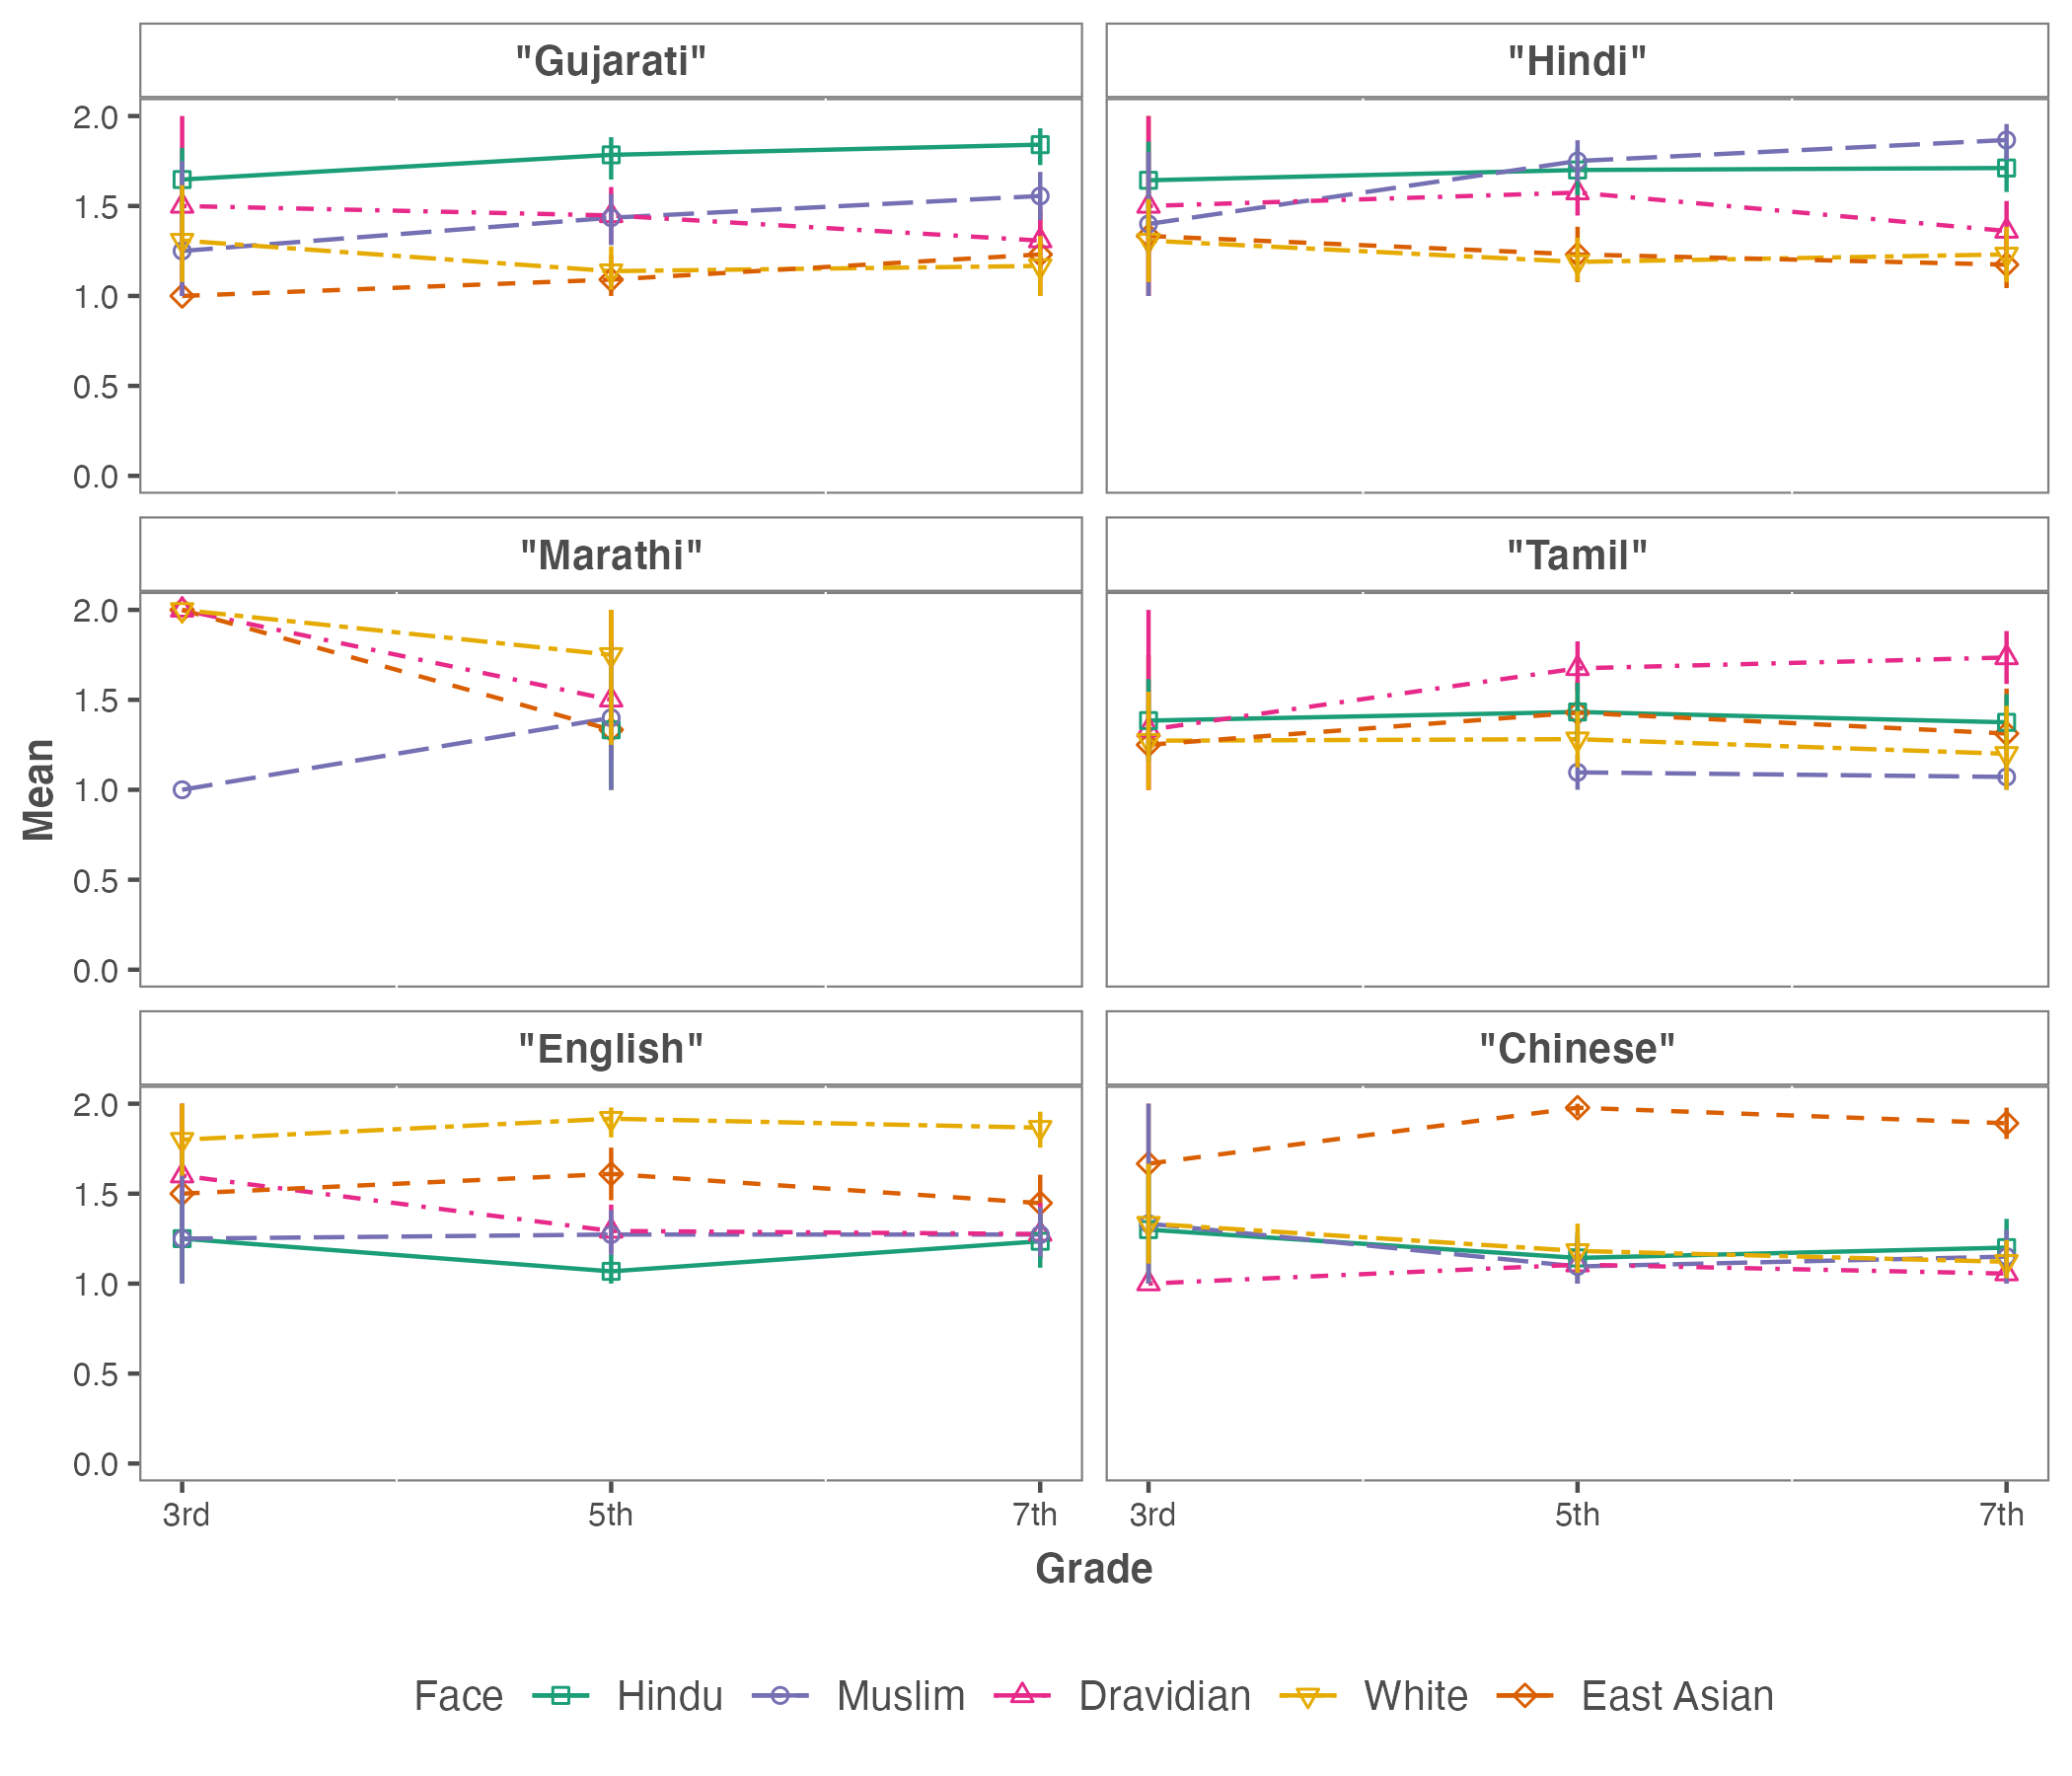
\includegraphics[width=\linewidth]{figures/std_plots/learning_faces_std.png}
%    \caption{\textit{Mean Predicted Learning \emph{(``How well will she come to learn---?'')} for Each Language and Face, by Grade.} Points plot mean rating (on a scale from 1--3) for each face (lines) by grade (x-axis), with error bars representing 95\% bootstrapped confidence intervals, in panels by language.}
%    \label{fig:faces-learning-score}
%\end{figure*}
\subsection*{Explicit Linguistic Essentialism Prompts}
\begin{figure}[h!]
    \centering
    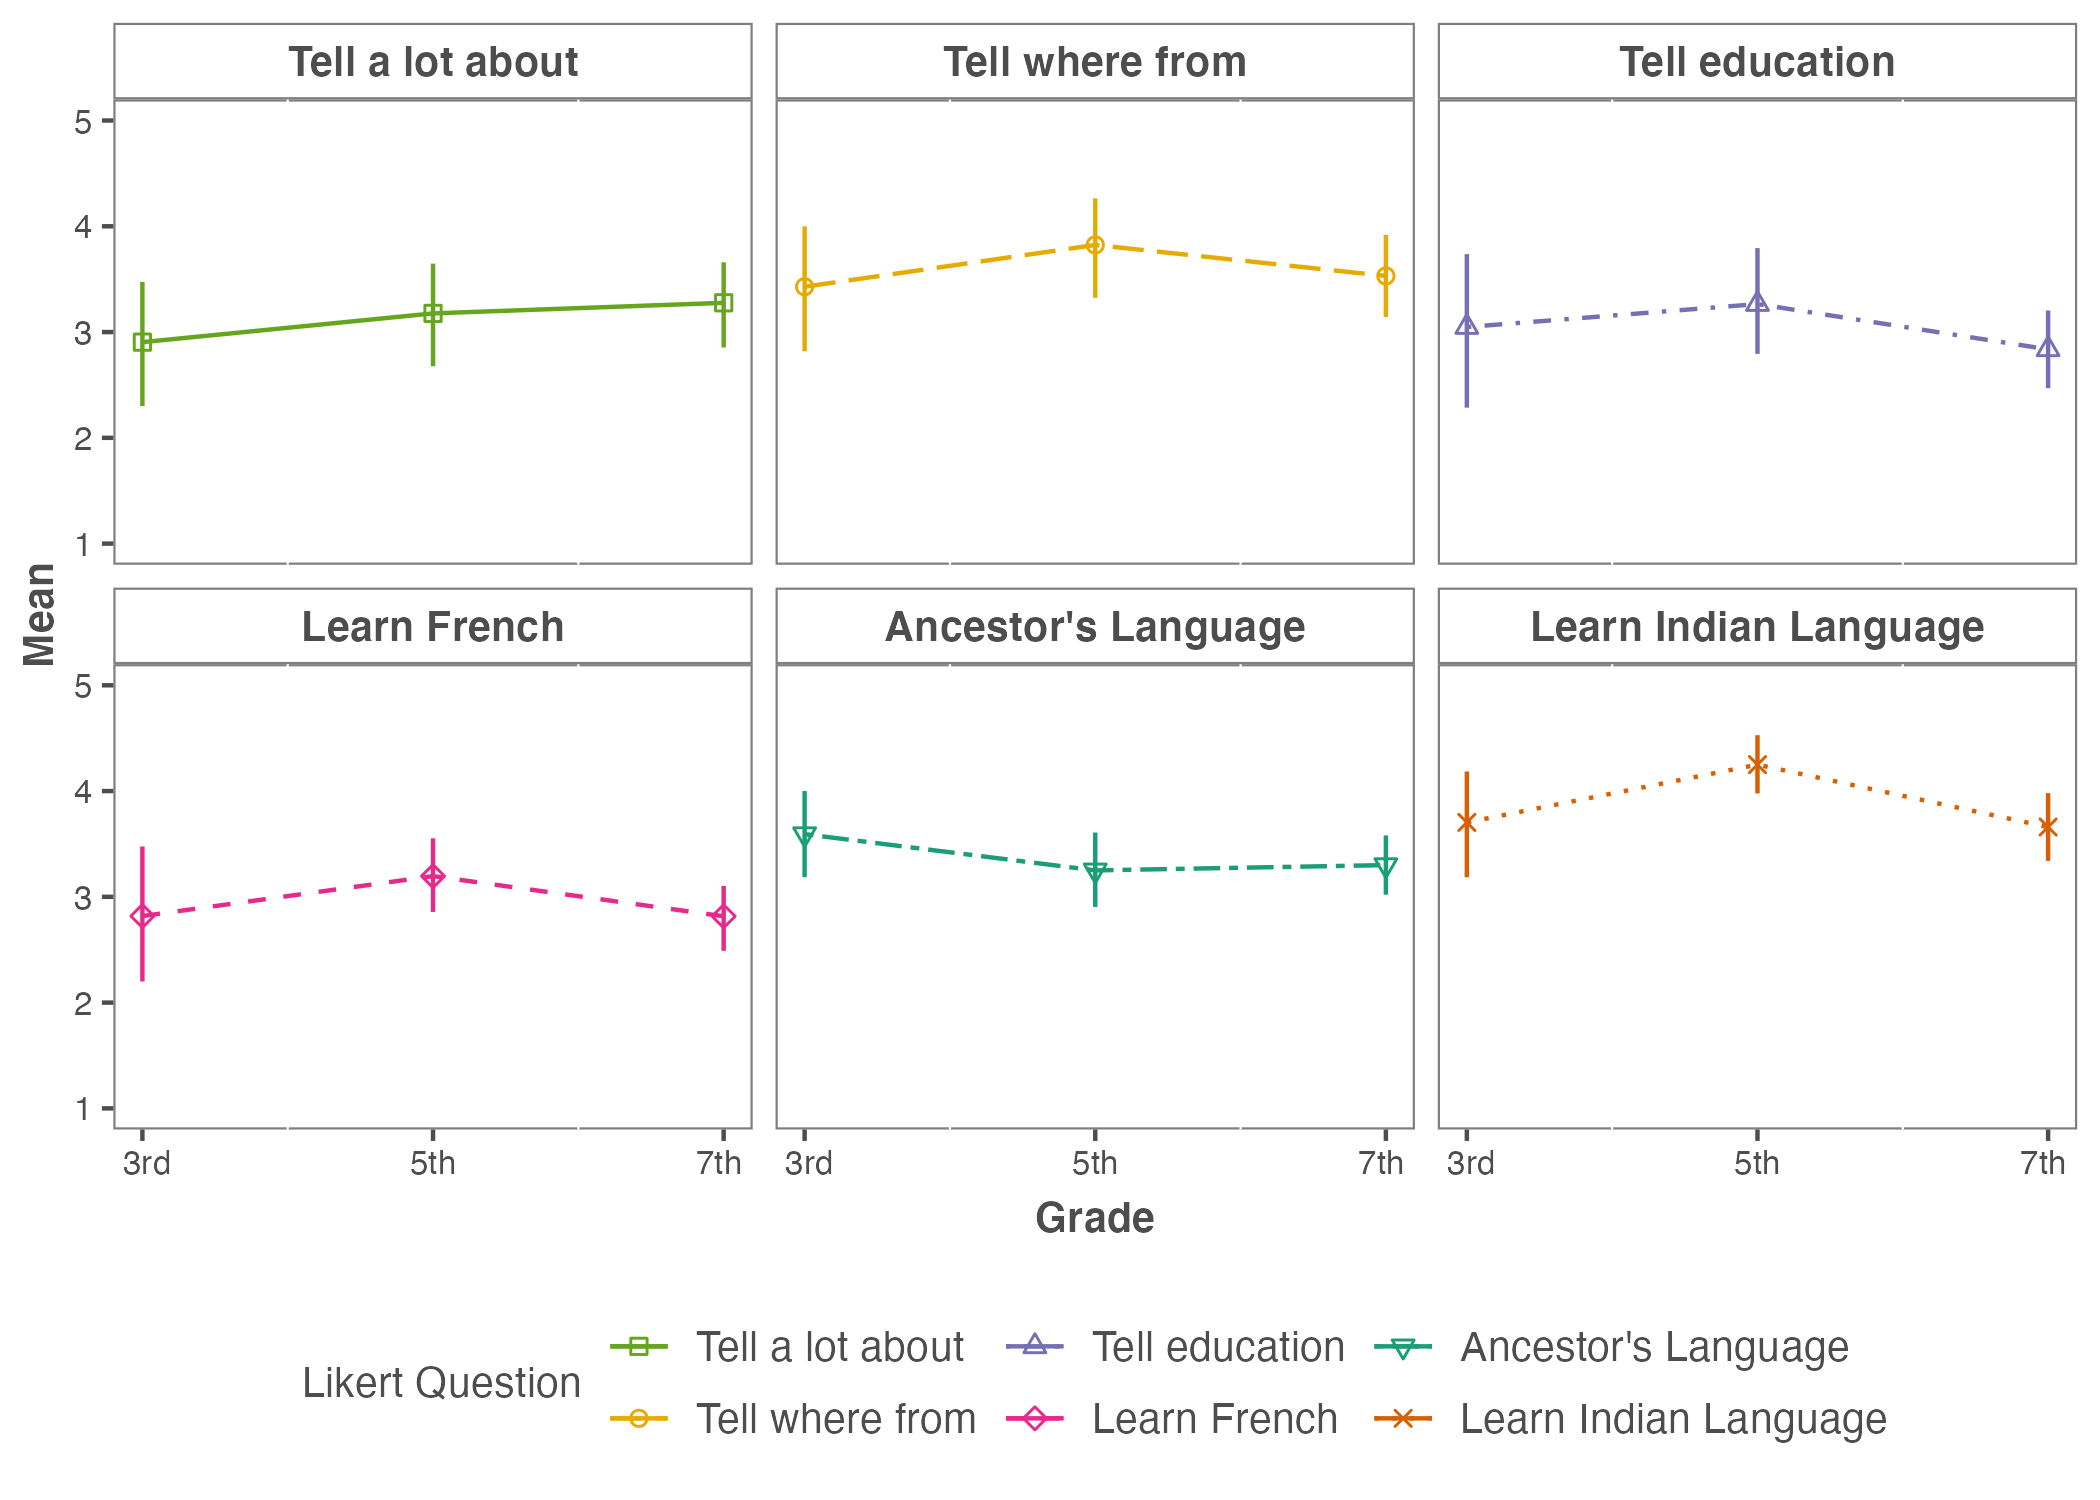
\includegraphics[width=\linewidth]{figures/std_plots/likert_std.png}
    \caption{\textit{Mean Responses to Likert Essentialism Prompts by Child Grade.} Points plot the mean of children's responses (on a scale from 1---\textit{Strongly Disagree} to 5---\textit{Strongly Agree}) at each grade, with error bars reflecting 95\% bootstrapped confidence intervals. 
    Panels display the selection rates for each question individually.}
    \label{fig:likert}
\end{figure}
%Link between language and religious/ethnic identity

Children additionally responded to a set of Likert-style items adapting and extending classic essentialism probes (items 1--3, below; %(e.g., ``It is easier to learn a language that was spoken by your ancestors than a language that was not spoken by your ancestors, even if no one in your family currently speaks it;'' see
\cite{gelman2007developmental, byers2015bilingualism, gelman1999biological}). Given the low intercorrelation between responses on these three items (Cronbach's $\alpha=0.035$), we did not analyze this method of accessing children's essentialist reasoning any further. 

We also measured children's agreement with more general statements about what can be assumed about a person from the languages they speak (items 4--6). %(e.g., ``You can tell how much education someone has had by the language(s) they speak.''). 
Children responded on a 5-point scale from ``Strongly Disagree'' to ``Strongly Agree,'' and justified their responses (these open-ended responses are not analyzed here). Mean responses to each question are plotted by child grade in Figure~\ref{fig:likert}. 
\begin{enumerate}[(1)]
    \item \textsc{Ancestors}: It is easier to learn a language that was spoken by your ancestors than a language that was not spoken by your ancestors, even if no one in your family currently speaks it. \textit{(Why?)}
    \item \textsc{India}: Imagine two people, one who is from India, one is not from India. It will be easier for the person from India originally to learn an Indian language (e.g., Gujarati, Hindi, Marathi), even if they do not live in India now, and do not know any other Indian languages. \textit{(Why?)}
    \item \textsc{French}: I could learn French as well as someone whose ancestors spoke French, but whose family lives in India and does not speak French. \textit{(Why?)}
    \item \textsc{Tell a lot}: You can tell a lot about a person by the language(s) they speak.  \textit{(Why?)}
    \item \textsc{Tell where from:} You can tell where a person is from by the language(s) they speak.  \textit{(Why?)}
    \item \textsc{Tell education:} You can tell how much education someone has had by the language(s) they speak.  \textit{(Why?)}
\end{enumerate}
\printbibliography
\end{document}